\documentclass[10pt]{amsart}
\usepackage[a4paper,margin=23mm]{geometry}
\usepackage{amsmath,amssymb,amsthm,mathtools,hyperref,float,enumitem,tikz}
\usetikzlibrary{decorations.pathmorphing,decorations.pathreplacing,decorations.shapes}
\setlist[1]{label=\textup{(\arabic*)}}
\newtheorem{thm}{Theorem}[section]
\newtheorem{pro}[thm]{Proposition}
\newtheorem{lem}[thm]{Lemma}
\newtheorem{cor}[thm]{Corollary}
\theoremstyle{definition}
\newtheorem{defi}[thm]{Definition}
\newtheorem{exa}[thm]{Example}
\newtheorem{ntn}[thm]{Notation}
\theoremstyle{remark}
\newtheorem{rem}[thm]{Remark}
\emergencystretch=3em

\newcommand\xuad{\hspace{2ex}}

\newcommand\nl{\par\noindent}

\newcommand\ssty{\scriptstyle}

\newcommand\ov{\overline}
\newcommand\un{\underline}
\newcommand\wh{\widehat}
\newcommand\wt{\widetilde}

\newcommand\mc{\mathcal}
\newcommand\mf{\mathfrak}

\newcommand\smeno{\smallsetminus}

\newcommand\nullvec{\underline 0}

\newcommand\nat{\mathbb N} 
\newcommand\ganz{\mathbb Z} 
\newcommand\real{\mathbb R}
\newcommand\compl{\mathbb C} 

\newcommand\pol{\mathcal P}
\newcommand\conv{\mathrm{Conv}}
\newcommand\cone{\mathrm{Cone}}

\newcommand\inc{\mathrm{Inc}}

\newcommand\gen{\mathrm{Span}}

\newcommand\Min{\mathrm{Min}}
\newcommand\Max{\mathrm{Max}}

\newcommand\supp{\mathrm{Supp}}
\newcommand\rk{\mathrm{rk}}
\newcommand\alt{\mathrm{ht}}

\newcommand\al{\alpha}
\newcommand\be{\beta}
\newcommand\ga{\gamma}
\newcommand\de{\delta}
\newcommand\ep{\varepsilon}
\newcommand\ka{\kappa}

\newcommand\comp{\lessgtr}
\newcommand\incomp{\not\lessgtr}

\newcommand\nosim{\not\sim}

\newcommand\red{\mathrm{Red}}

\newcommand\erm{{\mathrm{e}}}

\newcommand\preq{\preccurlyeq}

\renewcommand{\leq}{\leqslant}

%%%%%%%%%%%%%%%%%%%%%%%%%%%%%%%%%%%%

\title{Triangulations of standard parabolic facets of root polytopes}
\author{Paola Cellini}
\date{}
\begin{document}
\maketitle
\noindent\textbf{Source.} Theorem 1.1, Triangulations of root polytopes, Algebraic Combinatorics 1 (2018), 115--145, DOI 10.5802/alco.7. The original irreducible crystallographic hypotheses, facet-ideal and crossing-pair definitions, detachable/bipartition/triangulation orders and full case analyses, cone covering, linear independence and common-face intersection proofs are retained below. Additional source conclusions, including the lattice-volume theorem, are uncounted context. All authored mathematical TikZ diagrams remain editable; the publisher class and scripts are not used.
\section{Introduction}\label{sec:intro}

\par
Let $\Phi$ be an irreducible crystallographic root system in a Euclidean space $\mathrm E$, $\Phi^+$ a positive system of $\Phi$, and $W$ the Weyl group of $\Phi$. 
Then, let  $\pol$ be the {\it root polytope} associated with $\Phi$, i.e. the convex hull of all  roots in $\Phi$. 

\par 
In \cite{CM1}, Marietti and the author have studied a natural set of representatives of the faces of $\pol$ modulo the action of $W$, the {\it standard parabolic} faces of $\pol$.  
The set of all roots contained in a standard parabolic face is an abelian ideal of  $\Phi^+$ (see Subsection~\ref{ssec:adnilpotent} for a definition). 
We call {\it face ideals} or {\it facet ideals} the  abelian ideals of $\Phi^+$ corresponding to the standard parabolic faces or facets of $\pol$.

\par
In \cite{CM2}, for $\Phi$ of type $\mathrm A_n$ and $\mathrm C_n$,
the same authors have constructed a triangulation of the standard parabolic facets whose simplexes have a natural interpretation in terms of the corresponding facet ideals. 
The construction is formally equal for both root types, though the proofs are distinct and based on the special combinatorics of these two root systems and their maximal abelian ideals.  
Through the action of $W,$ a triangulation of all the standard parabolic facets can be extended to a triangulation of the boundary of $\pol$. 
Such an extension corresponds to an appropriate choice of representatives of the left cosets of $W$ modulo  the stabilizers of the standard parabolic facets.
The triangulations of the boundary of $\pol$ are also studied in  \cite{Ard} for all classical root types, using the coordinate description of $\Phi$.
In \cite{GGP}, the triangulations of the positive root polytope $\pol^+$, i.e the convex hull of the positive roots and the origin,  are studied for $\Phi$ of type $\mathrm A_n$.
The triangulations of $\pol^+$ are also studied in \cite{Mesz1, Mesz2} for $\mathrm A_n$ and $\mathrm C_n$.

\par
In this paper, we give a uniform construction of a triangulation of the standard parabolic facets,  for all finite irreducible crystallographic root systems. 
The construction coincides with the one of \cite{CM2} for the types $\mathrm A_n$ and $\mathrm C_n$.  
We also obtain unimodularity results similar to those obtained for $\mathrm A_n$ and $\mathrm C_n$.  

\par
We need some preliminaries for describing the results in more detail.
If $\be_1$, $\be_2$, $\ga_1$, $\ga_2\in \Phi^+$ are such that $\be_1+\be_2=\ga_1+\ga_2$, we say that $\{\be_1, \be_2\}$ and $\{\ga_1, \ga_2\}$ are {\it crossing pairs}. 
We first prove that if $\{\be_1,\be_2\}, \{\ga_1, \ga_2\}$ are crossing pairs contained in a (common) abelian ideal,  then, for all $i, j$ in $\{1, 2\}$, the differences $\be_i-\ga_j$ are roots, in particular  $\be_i$ and $\ga_j$ are comparable. 
This implies that the set $\{\be_1,\be_2, \ga_1, \ga_2\}$ has a minimum and a maximum, more precisely, one of the two crossing pairs consists of these minimum and maximum, i.e., either $\be_1< \ga_i< \be_2$ for both $i=1$ and $2$, or the analogous relation with $\be$ and $\ga$ interchanged holds.
We define the relations $\lesssim$ and $\sim$ on $\Phi^+$ as follows.
For all $\be_1, \be_2$ in $\Phi^+$, we write $\be_1\lesssim \be_2$ if there exist 
$\ga_1, \ga_2$ such that $\be_1+\be_2=\ga_1+\ga_2$ and $\be_1< \ga_i< \be_2$ for both $i=1$ and $2$. 
Moreover, we write $\be_1\sim \be_2$ if $\be_1\lesssim \be_2$ or $\be_2\lesssim \be_1$.
Finally, we say that a subset $R$ of $\Phi^+$ is {\it reduced} if $\be_1\nosim \be_2$ for all $\be_1, \be_2\in R$.  

\par
The first main result in this paper is that the maximal reduced subsets in a facet ideal provide a triangulation of the corresponding standard parabolic facet.
For each standard parabolic facet $F$ of $\pol$, let $I_F$ be the corresponding facet ideal:
$$
I_F=F\cap \Phi,
$$
and
$$
\mc T_F=\{\conv(R)\mid R\subseteq I_F,\ R \text { maximal reduced\,}\},
$$
where $\conv(R)$ is the convex hull of $R$. 
Then the following result holds.

\begin{thm}\label{thm:main1-intro}
For each standard parabolic facet  $F$ of $\pol$,  $\mc T_F$ is a triangulation of $F$.
\end{thm}

\par
Clearly, the set of vertexes of the above triangulation is the set of all roots contained in~$F$. 

\par
Theorem~\ref{thm:main1-intro} implies, in particular, that the maximal reduced subsets in $I_F$ are linear bases of $\mathrm E$. 
Let $\Pi$ and $\theta$ be the simple system and the highest root of $\Phi^+$. 
Then, $\{-\theta\}\cup \Pi$ is the set of vertexes of the affine Dynkin diagram of $\Phi$.
For each $\al\in \Pi$,  let $\Phi_{\al}$ and $\wh\Phi_{\al}$ be the root subsystems of $\Phi$ generated by $\Pi\smeno\{\al\}$ and  $\{-\theta\}\cup (\Pi\smeno\{\al\})$, respectively, and $\Phi_\al^+$ and $\wh\Phi_{\al}^+$ their positive systems contained in $\Phi^+$.
Clearly, $\wh\Phi_{\al}$ has the same rank as $\Phi$.
We call the $\wh\Phi_\al$, for all $\al\in \Pi$, the {\it standard equal rank} subsystems of $\Phi$.
The standard parabolic facets of $\pol$ naturally correspond to the {\it irreducible} standard equal rank root  subsystems of $\Phi$ \cite{CM1}. 
Precisely, for each $\al\in \Pi$ such that $\wh\Phi_{\al}$ is irreducible,  let
$$
I_\al=\wh\Phi_{\al}^+\smeno \Phi_\al.
$$ 
Then $I_\al$ is a facet ideal of $\Phi^+$, and each facet ideal of $\Phi^+$ is obtained in this way (see Subsection~\ref{ssec:faces}). We prove the following result.


\begin{thm}\label{thm:main2-intro}
Let $\al\in \Pi$ be such that $\wh\Phi_{\al}$ is irreducible.
Then, each  maximal reduced subset contained in the facet ideal $I_\al$ is a $\ganz$-basis of the root lattice of $\wh\Phi_{\al}$.  
In particular, all the simplexes of the triangulation  $\mc T_F$  have the same volume.
\end{thm}


\par
Part of the proofs require a case by case analysis. 
The cases to be considered can be restricted to a special, proper subset of facet ideals. 
Indeed, the results of \cite{CM1} imply that the facet ideal  $I_\al$  ($\al\in \Pi$,  $\wh\Phi_{\al}$ irreducible), is an {\it abelian nilradical} (see Subsection~\ref{ssec:abnil}) in the root subsystem $\wh\Phi_\al^+$.  
Hence, we may reduce to the case of abelian nilradicals.

\par
The case by case analysis is contained in the proof of Proposition~\ref{pro:tri-ord-existence}.
This proof also provides an algorithm for the explicit computation of the triangulations for each root type, which will be done in a future paper. 

\section{Preliminaries}\label{sec:preli}

In this section we fix our main notation and recall some preliminary results. 
For the basic preliminary notions, we refer to \cite{Bou} and \cite{HuCox} for root systems, and to \cite{Bou2} and \cite{HuLie} for Lie algebras. 


\subsection{Basic notation}\label{ssec:basic-not}
{\sl General.} We sometimes use the symbol $:=$ for emphasizing  that equality holds by definition or that we are defining the left term of equality.
We denote by $\mathrm E$ a Euclidean space, with scalar product  $(\cdot \,,\cdot )$ and norm $|\cdot |$. We identify $\mathrm E$ with its dual space, through $(\cdot \,,\cdot)$. The null vector of $\mathrm E$ is denoted by $\nullvec$. 
For any $S\subseteq \mathrm E$, $\gen(S)$ is the vector subspace generated by $S$ over $\real$ (the field of real numbers), and $\rk(S):=\dim\gen(S)$.

\par
{\sl Root systems.}
We denote by $\Phi$ a reduced irreducible crystallographic root system in $\mathrm E$ and by $\Phi^+$ a fixed positive system of $\Phi$.
The simple system of $\Phi$ corresponding to  $\Phi^+$ is denoted by $\Pi$,  while $\Omega^\vee$ is the set of fundamental co-weights of $\Phi$, i.e., the  dual basis of $\Pi$ in $\mathrm E$.  
For each $\al\in \Pi$, $\check\omega_\al$ is the fundamental co-weight  defined by the conditions $(\al, \check\omega_\al)=1$ and $(\al', \check \omega_\al)=0$ for all $\al'\in \Pi\smeno \{\al\}$. 
For all $\al\in \Pi$ and $\be \in \Phi$, we set $c_\al(\be)=(\be, \check\omega_\al)$, so that  
$$\be=\sum\limits_{\al\in\Pi}c_\al(\be)\al.$$
The {\it support} of $\be$ is the set of simple roots with non-zero coefficient in the expression of~$\be$: 
$$
\supp(\be)=\{\al\in \Pi\mid c_\al(\be)\neq 0\}.$$
The highest root in $\Phi^+$ is denoted by $\theta$ and its coefficients with respect  to $\Pi$ by $m_\al$, thus
$$\theta=\sum\limits_{\al\in \Pi} m_\al\al.$$ 
We call $m_\al$ the {\it multiplicity of $\al$ in $\Phi^+$}.

\par
For all $\be\in \Phi$, $\be^\vee$ is the corresponding coroot, i.e., $\be^\vee=\frac{2\be}{(\be, \be)}$.

\par
For each root subsystem $\Psi$ of $\Phi$ we set $\Psi^+=\Psi\cap \Phi^+$. 
It is well known that $\Psi^+$ is a positive system for $\Psi$: we call it the {\it standard positive system} of $ \Psi$.
Moreover, we denote by $L(\Psi)$ and $L^+(\Psi)$ the root lattice and positive root lattice of $\Psi$, i.e. the $\ganz$-span of $\Psi$ and the $\nat$-span of $\Psi^+$, respectively, where $\ganz$ and $\nat$ are the sets of integers and non-negative integers. 

\par
For any $S\subseteq \Phi$, we denote by $\Phi(S)$ the root subsystem of $\Phi$ generated by $S$, i.e., the minimal root system containing $S$, and we write  $\Phi^+(S)$ for $\Phi(S)^+$. 

\par
A root subsystem $\Psi$  of $\Phi$ is called {\it parabolic} if
$\Psi=\Phi\cap \gen(\Psi)$.  
For any linear subspace $H$ of $E$, the intersection $\Phi\cap H$ is a parabolic root subsystem.
Hence, $\Psi$ is a parabolic subsystem of $\Phi$ if and only if there exists a linear subspace $H$ of $E$ such that $\Psi=\Phi\cap H$.

\par
{\sl Posets.} As usual, $\leq$ denotes  both the order of $\real$ and the partial order of $\mathrm E$ associated to $\Phi^+$:  for all $x,y\in \mathrm E$,  $x\leq y$ if and only if $y-x\in L^+(\Phi)$.
We call this last order {\it the  standard partial order}.
We will need only the restriction of the standard partial order to $\Phi^+$. 
For any $S\subseteq \Phi^+$, we denote by $\Min\,S$ and $\Max\, S$, with capital M, the sets of minimal and maximal elements of $S$, and by $\min S$ and $\max S$ its possible minimum and maximum, with respect to $\leq$. 
The analogous objects with respect to any other order relation $\preq$, will be distinguished by adding the subscript~$\preq$.
The elements in  $\Min\,S\cup \Max\, S$ are called {\it the extremal} elements of $S$.
We say that $S$  is {\it saturated} if it is saturated with respect to the standard partial order, i.e., for all $\be_1, \be_2\in S$ such that $\be_1\leq \be_2$, all the interval $[\be_1, \be_2]:=\{\ga\in \Phi \mid \be_1\leq \ga\leq \be_2\}$ is contained in $S$.
Any subset $S'$ of $S$ is called {\it an initial section of $S$} if for all $\be\in S'$ and $\ga\in S$, if $\ga \leq \be$, then $\ga \in S'$. 
The final sections are defined similarly. 
Then, $S'$ is an initial section of $S$ if and only if $S\smeno S'$ is a final section of $S$.

\par
For any order relation $\preq$ on $\Phi^+$ and for all $\be\in \Phi^+$, we denote $(\be^\preq)$ the {\it $\preq$-upper cone of} $\be$, i.e., 
$$(\be^\preq)=\{\ga\in \Phi^+\mid \be\preq \ga\}.$$  
Clearly, this is a {\it dual order ideal}, or {\it filter},  in the poset $(\Phi^+,\preq)$.


\subsection{Basic lemmas on roots}\label{ssec:basic-roots}
\subsubsection{General facts}\label{sssec:general-roots}
We first recall some  basic facts that we will use also without explicit mention. 
Since we are assuming $\Phi$ irreducible and reduced, the lengths of roots in $\Phi$ are at most $2$ \cite[Ch.~VI, \S~1.4]{Bou}. 
We denote by $\Phi_\ell$ the set of roots of maximal length ({\it long roots}), and set $\Phi_s=\Phi\smeno\Phi_\ell$ (the set of {\it short roots}). 
By definition, if only one length occurs, all roots are long.
Results \ref{itm:obtuse-are-summable} to \ref{itm:simple-obtuse}
below can be found in  \cite[Ch.~VI, \S~1, n.~3, 4, 5]{Bou}.
%\smallskip

\begin{enumerate}
\item
For all $\be, \ga\in \Phi$, if $(\be, \ga)<0$ and $\be\neq -\ga$, then $\be+\ga\in \Phi$. Equivalently, if $(\be, \ga)>0$ and $\be\neq \ga$, then $\be-\ga\in \Phi$.
\label{itm:obtuse-are-summable}
\item
For all $\be, \ga\in \Phi$, if $\be\neq \ga$ and  either $\ga\in \Phi_\ell$, or $|\be|=|\ga|$, then $(\be, \ga^\vee)\in \{0, \pm 1\}$. 
If $|\be|>|\ga|$, then $\frac{(\be, \be)}{(\ga, \ga)}\in \{2, 3\}$ and $(\be, \ga^\vee)=
\frac{(\be,\be)}{(\ga,\ga)}(\be^\vee, \ga)
\in \{0, \pm 2, \pm 3\}$. 
\label{itm:length-ratio}
\item
For all $\be, \ga\in \Phi$, the set $I=\{k\in \ganz\mid \be+k\ga\in \Phi\}$ is a an interval of $\ganz$. 
\label{itm:root-string}
\item
For all $\al, \al'\in \Pi$, $(\al, \al')\leq 0$.
\label{itm:simple-obtuse}
%\par\noindent
\end{enumerate}
%\smallskip

We note that in (2), since the root lengths are at most two, we have either  $\frac{(\be,\be)}{(\ga,\ga)}=2$ and $(\be, \ga^\vee)\in \{0,\pm2\}$ for all $\be, \ga\in \Phi$ such that  $|\be|>|\ga|$, or $\frac{(\be,\be)}{(\ga,\ga)}=3$ and $(\be, \ga^\vee)\in \{0,\pm 3\}$ for all $\be, \ga\in \Phi$  such that $|\be|>|\ga|$.

\subsubsection{Summable roots}\label{sssec:summable-roots}
Next proposition contains a less known result.
The proof requires some basic notions and results from Lie theory.
Let $\mf g$ be  a complex simple Lie algebra with root system $\Phi$ with respect to the Cartan subalgebra $\mf h$ (see e.g. \cite[\S 18]{HuLie}). 
Thus, $\mf g=\left(\bigoplus_{\al\in\Phi}\mf g_\al\right)\oplus \mf h$, where $\mf g_\al$ is the root space of $\al$,  for all $\al\in \Phi$, and  $\left(\gen_\compl(\Phi)\right)=\mf h^*$, the dual space of $\mf h$. 

\par
We say that two roots are {\it summable} if their sum is a root.
It is well known that if $\al$ and $\be$ are summable roots, then $[\mf g_\al,\mf g_\be]=\mf g_{\al+\be}$, while if  $\al$ and $\be$ are not summable and $\al\neq -\be$, then  $[\mf g_\al,\mf g_\be]=\{\nullvec\}$. 

\begin{pro}\label{pro:smart}
Let $\be_1, \be_2, \be_3\in  \Phi$ be such that $\be_1+\be_2+\be_3\in \Phi$  and $\be_i\neq -\be_j$ for all $i, j\in\{1, 2, 3\}$.
Then at least two of the three sums $\be_i+\be_j$, with $i, j\in\{1, 2, 3\}$ and $i\neq j$, belong to $\Phi$.
\end{pro}

\begin{proof}
For all $i\in \{1, 2, 3\}$, we have $\be_1+\be_2+\be_3\neq \be_i$, otherwise, for $\{j, k\}=\{1, 2, 3\}\smeno\{i\}$, we have $\be_j+\be_k=\nullvec$, contrary to the assumption.
Moreover, for at least one $i\in \{1, 2, 3\}$ we have $(\be_1+\be_2+\be_3, \be_i)>0$, since $(\be_1+\be_2+\be_3, \be_1+\be_2+\be_3)>0$,  hence  $\be_1+\be_2+\be_3- \be_i\in \Phi$. 
Assume for example $\be_1+\be_2\in \Phi$. 
Then, $[[\mf g_{\be_1}, \mf g_{\be_2}],\mf g_{\be_3}]=[\mf g_{\be_1+\be_2},\mf g_{\be_3}]=\mf g_{\be_1+\be_2+\be_3}\neq \{\nullvec\}$, hence, by the Jacobi identity, at least one of $[[\mf g_{\be_1}, \mf g_{\be_3}],\mf g_{\be_2}]$ 
and $[\mf g_{\be_1}, [\mf g_{\be_2},\mf g_{\be_3}]]$ is non zero. It follows that at least one of $\be_1+\be_3$ and $\be_2+\be_3$ is a root.
\end{proof}
%\smallskip

\par
As we have recalled, if two roots have strictly negative scalar product, then they are summable. 
The reverse implication holds if $\Phi$ is simply laced, but is false in general, as we see in the following lemma, where the Cartan integers of pairs of summable roots are classified. 

\pagebreak

\begin{lem}\label{lem:esercizio}
Assume $\be, \ga, \be+\ga\in \Phi$. 
\begin{enumerate}
\item
If $|\be|=|\ga|=|\be+\ga|$, then $(\be, \ga^\vee)=-1$.
\label{itm:all-equal-lengths}
\item
If $|\be|=|\ga|\neq |\be+\ga|$, then either 
$\frac{|\be+\ga|^2}{ |\be|^2}= 2$ and  $(\be, \ga^\vee)=0$, or $\frac{|\be+\ga|^2}{ |\be|^2}=3$ and  $(\be, \ga^\vee)=1$. 
In any case, $|\be|=| \ga|< |\be+\ga|$.
\label{itm:equal-lengths-summands}
\item
If $|\be|<|\ga|$, then $|\be+\ga|=|\be|$, $(\be^\vee,\ga)=-\frac{|\ga|^2}{ |\be|^2}\in \{-2, -3\}$, and  $(\be, \ga^\vee)=-1$.  
\label{itm:two-lengths-summands}
\end{enumerate}
\end{lem}

\begin{proof}
\ref{itm:all-equal-lengths} and \ref{itm:equal-lengths-summands}. 
Since $|\be|=|\ga|$, we have $\frac{|\be+\ga|^2}{ |\ga|^2}= \frac{(\be,\be)+2(\be,\ga)+(\ga,\ga)}{(\ga,\ga)}=2+\frac{2(\be,\ga)}{(\ga,\ga)}=2+(\be,\ga^\vee)$. 
Moreover, in case (1) we have $\frac{|\be+\ga|^2}{ |\ga|^2}=1$, while in case (2) we have $\frac{|\be+\ga|^2}{ |\ga|^2}=\frac{|\be+\ga|^2}{ |\be|^2}\in \{2, 3\}$. 
In all cases, the claim follows directly. 

\par
\ref{itm:two-lengths-summands} If $|\be+\ga|=|\ga|$, we get $1=\frac{|\be+\ga|^2}{ |\ga|^2}= \frac{(\be,\be)}{(\ga, \ga)}+(\be,\ga^\vee)+1$, hence $\frac{(\be,\be)}{(\ga, \ga)}=-(\be,\ga^\vee)\in \ganz$, contrary to the assumption.
Hence, $|\be+\ga|=|\be|$, and $1=\frac{|\be+\ga|^2}{ |\be|^2}= 1+(\be^\vee,\ga)+\frac{|\ga|^2}{ |\be|^2}$.
Hence, $(\be^\vee,\ga)=-\frac{|\ga|^2}{ |\be|^2}\in \{-2, -3\}$.
Finally, since $(\be,\ga^\vee)=\frac{ |\be|^2}{|\ga|^2}\,(\be^\vee,\ga)$, we have $(\be,\ga^\vee)=-1$
\end{proof}
\medskip

\par
The assumptions of parts \ref{itm:all-equal-lengths}, \ref{itm:equal-lengths-summands}, and \ref{itm:two-lengths-summands} of Lemma~\ref{lem:esercizio} are mutually exclusive and cover all possibilities for the relations among $|\be|$, $|\ga|$, and  $|\be+\ga|$.  
In particular, if $\be$ and $\ga$ have nonnegative scalar product, then, by parts \ref{itm:all-equal-lengths} and \ref{itm:two-lengths-summands}, we obtain that the assumptions of part \ref{itm:equal-lengths-summands} holds. 
Similarly, if $\ga$ is long, then the assumptions of parts \ref{itm:all-equal-lengths} or \ref{itm:two-lengths-summands} hold.
Hence, we obtain the following proposition. 

\begin{pro}\label{pro:summable-acute}
For all $\be, \ga\in \Phi$, the following results holds.
\begin{enumerate}
\item 
If $\be$ and $\ga$ are summable, then  we have 
$(\be, \ga)\geq 0$ if and only if $|\be|= | \ga|<|\be+\ga|$.
\label{itm:general}
\item
If $\ga\in \Phi_\ell$, then $\be$ and $\ga$ are summable if and only if $(\be, \ga^\vee)=-1$.
\label{itm:long}
\end{enumerate}
\end{pro}
%\smallskip

\subsection{Ad-nilpotent and abelian ideals}\label{ssec:adnilpotent}

\par
Let $\mf g$ be as in Subsection~\ref{ssec:basic-roots}, 
$\mf b$ be the standard Borel subalgebra of $\mf g$ associated to $\Phi^+$,  and $\mf n$ its nilpotent radical, i.e., $\mf b=\left(\bigoplus_{\al\in\Phi^+}\mf g_\al\right)\oplus \mf h$ and $\mf n=\bigoplus_{\al\in\Phi^+}\mf g_\al$. 

\par
An {\it ad-nilpotent} ideal of $\mf b$ is a (nilpotent) ideal of $\mf b$ contained in $\mf n$. 
Being $\mf h$-stable, such an ideal is a sum of root spaces.
For any $I\subseteq \Phi^+$, the sum of root spaces $\bigoplus_{\al\in I} \mf g_\al$ is an ad-nilpotent ideal of $\mf b$ if and only if, for all $\al, \beta\in \Phi^+$, if $\al\in I$ and $\al\leq \beta$, then $\beta\in I$. 
A subset $I$ of $\Phi^+$ with this property is called an {\it ad-nilpotent ideal} of $\Phi^+$.
Thus, an ad-nilpotent ideal of $\Phi^+$ is a filter in $(\Phi^+, \leq)$, i.e. a dual order ideal. 
It is easy to see that an abelian ideal of $\mf b$ must be ad-nilpotent. 
For any  $I\subseteq \Phi^+$, the subspace $\bigoplus_{\al\in I} \mf g_\al$ is an abelian ideal of $\mf b$ if and only if $I$ is an ad-nilpotent ideal of $\Phi^+$ with the further property that, for all $\al, \beta\in I$, $\al+\beta\not\in \Phi$. 
Such an $I$ is called an {\it abelian ideal} of $\Phi^+$.
The  abelian ideals of $\Phi^+$ are studied in several papers, both for their implications in representation theory and for their algebraic-combinatorial interest. 
The main representation theoretic motivations  can be found in \cite{Ko1, Ko2} (see also \cite{CMP}); the basic algebraic-combinatorial results can be found in \cite{CPadnilp1, CPab, Pan, Su}.


\subsection{Abelian nilradicals}\label{ssec:abnil}

\par
An ad-nilpotent ideal of $\Phi^+$ is called {\it principal} if it has a minimum, i.e. if the corresponding $\mf b$-ideal is principal. 
For all $\be\in \Phi^+$, the upper $\leq$-cone of $\be$, $(\be^\leq)=\{\ga\in \Phi^+\mid \be\leq \ga\}$, is also called the principal ad-nilpotent ideal {\it generated} by $\be$.  
It is clear that if $\be\in \Phi^+$ is such that $c_\al(\be)>\frac{m_\al}{2}$ for some $\al\in \Pi$, then $(\be^\leq)$ is abelian. 
In particular, this happens if $\be$ is a simple root of  multiplicity $1$ in $\Phi^+$. 
Indeed, the following well known result holds. 
For completeness, we include a proof.
\par

\begin{pro}\label{pro:simple-principal}
Let $S\subseteq\Pi$ and $I=\Phi^+\smeno \Phi(S)$. 
Then $I$ is an ad-nilpotent ideal. 
Moreover, $I$ is abelian if and only if either $S=\Pi$, or $S=\Pi\smeno\{\al\} $ for  a simple root $\al$ such that $m_\al=1$. 
In this case, $I$ is equal to $(\alpha^\leq)$ and is a maximal abelian ideal.
\end{pro}

\begin{proof}
It is immediate that  $I$ is an ad-nilpotent ideal. 
If $S=\Pi$, then $I$ is the empty root ideal, hence it is abelian. 
Let  $S=\Pi\smeno \{\al\}$ with $\al\in \Pi$ and $m_\al=1$. 
Then, by definition we have $I=(\al^\leq)$, which is abelian  since $m_\al=1$.
We prove that $(\al^\leq)$ is maximal abelian. 
If $S= \emptyset$, i.e. $\Pi=\{\al\}$,  then $I=\Phi^+$ and the claim is obvious. 
Let $S\neq \emptyset$ and let $J$ be an ad-nilpotent ideal that strictly contains $(\al^\leq)$.
We have to prove that $J$ is not abelian. 
By definition, there exists $\be\in J$ such that $\al\not\in\supp(\be)$.
Let $\Psi_1, \dots, \Psi_k$ be the irreducible components of $\Phi(\Pi\smeno \{\al\})$. 
Assume, for example, $\be\in \Psi_1$. 
Then, if  $\theta_1$ is the highest root of $\Psi_1$, we obtain $\theta_1\in J$.  
Let $S_1=\Psi_1\cap (\Pi\smeno\{\al\})$.
It is easily seen that, since $\Phi$ is irreducible, $\al$ cannot be orthogonal to the whole $S_1$. 
Hence, since $(\al, \al')\leq 0$ for all $\al'\in S_1$, there exists $\al'\in S_1$ such that $(\al',\al)< 0$. 
But $\supp(\theta_1)=S_1$, hence $(\theta_1,\al)\leq (\al', \al)< 0$. It follows that $\theta_1+\al\in \Phi$, and hence $J$ is not abelian.  

\par
It remains to prove the \lq\lq only if\rq\rq\ part. 
For all $\be\in \Phi$, let $\alt_{\Pi\smeno S}(\be)=\sum\limits_{\al\in\Pi\smeno S}c_\al(\be)$.
We have $S=\Pi$ if and only if  $\max\,\{\alt_{\Pi\smeno S}(\be)\mid\be\in \Phi\}=0$.
Similarly, we have $S=\Pi\smeno \{\al\}$ and $m_\al=1$ if and only if  $\max\,\{\alt_{\Pi\smeno S}(\be)\mid\be\in \Phi\}= 1$.
In order to conclude the proof, we assume $\max\{\alt_{\Pi\smeno S}(\be)\mid\be\in \Phi\}> 1$ and  prove that in this case $I$ is not abelian.
By definition, we have $\be\in I$ if and only if  $\alt_{\Pi\smeno S}(\be)>0$.
Let $\be^*\in \Min\{\be\in \Phi \mid \alt_{\Pi\smeno S}(\be)>1\}$. 
Since $(\be^*, \be^*)> 0$, there exists $\al\in \supp(\be^*)$ such that $(\be^*, \al)>0$, hence $\be^*-\al\in \Phi$, by \ref{sssec:general-roots}\ref{itm:obtuse-are-summable}. 
Such an $\al$ cannot belong to $S$, otherwise $\alt_{\Pi\smeno S}(\be^*-\al)=\alt_{\Pi\smeno S}(\be^*)$, contrary to minimality of $\be^*$. 
It follows $\al\in \Pi\smeno S$, hence $\al\in I$.
Now, $\be^*-\al\in I$, too, since $\alt_{\Pi\smeno S}(\be^*-\al)=\alt(\be^*)-1>0$, hence we obtain that $I$ is not abelian since $\al$ and $\be^*-\al$ are summable. 
\end{proof}

\par
For each $S\subseteq \Pi$, the ideal $\bigoplus\limits_{\al\in \Phi^+\smeno \Phi(S)}\mf g_\al$ is the nilradical (the largest nilpotent ideal) of the standard parabolic subalgebra  associated to $S$ (see \cite[Ch.~VIII, \S~3.4]{Bou2}). 
Hence, we call the maximal abelian ideals $(\al^\leq)$ with $m_\al=1$, together  with the empty root ideal, {\it the abelian nilradicals}. 

\subsection{The faces of the root polytope}\label{ssec:faces}
We recall some ideas and results from~\cite{CM1}. 
For all $\al\in \Pi$ and  all nonempty $S\subseteq \Pi$,  let
$$
H_{\al, m_\al}=\{x\in E\mid(x, \check\omega_\al)=m_\al\}, \qquad 
\mathrm F_\al=H_{\al, m_\al}\cap \pol,
\qquad
\mathrm F_S=\bigcap_{\al\in S} \mathrm F_\al.
$$

By definition of $m_\al$, we have $(\be, \check\omega_\al)\leq m_\al$ for all $\be\in \Phi$ and, therefore, $(x, \check\omega_\al)\leq m_\al$ for all $x\in \pol$. 
Hence, the affine hyperplanes $H_{\al, m_\al}$ are supporting hyperplanes of $\pol$, and the $\mathrm F_\al$ and  $\mathrm F_S$ are faces of $\pol$.  
We call them the {\it standard parabolic faces}. 
In fact, the set of all standard parabolic faces is a set of representatives of the orbits of  the action of the Weyl group $W$  on the set of proper faces of $\pol$ \cite{CM1} . 

\par
For each standard parabolic face $F$, let 
$$
I_F=F \cap \Phi.
$$
By definition,  for each nonempty $S\subseteq \Pi$, $I_{\mathrm F_S}$ is the set of all roots $\be$ such that $c_\al(\be)=m_\al$, for all $\al\in S$. 
It is easy to see that $\pol$ is the convex hull of the long roots (see  e.g. \cite{CM3}), hence the long roots in $I_{\mathrm F_S}$ are the vertexes of the face $\mathrm F_S$. 
\par

We recall that the {\it extended} Dynkin graph of $\Phi$ is obtained from the usual Dynkin graph by extending the vertex set $\Pi$ with $-\theta$ and completing the edge set according to the scalar products and the relative lengths between $-\theta$ and the roots in $\Pi$, with the same rules  used of the usual Dynkin graph.
For our purposes, it is convenient to consider the extended Dynkin graph on the opposite vertex set, i.e., $\{\theta\}\cup -\Pi$. 
This does not change the edges. 
We call the resulting graph the {\it opposite} extended Dynkin graph.
\par

For each $\Sigma\subseteq\Pi$, we set
$$ \Sigma^\erm=\{\theta\}\cup  -\Sigma.$$ 
Let $\Phi(\Sigma^\erm)$ be the root subsystem of $\Phi$ generated by $\Sigma^\erm$. 
For studying the face $F_S$, we need considering $\Phi(\Sigma^\erm)$ with $\Sigma=\Pi\smeno S$. 
In this case, $\Sigma\subsetneqq\Pi$, since $S$ is assumed to be nonempty.
(We point out that, contrary to what is done in \cite{CM1}, we are not making use of the affine root system associated to $\Phi$ and all root subsystems we are defining are inside~$\Phi$.)

It is well known that, if $\Sigma\subsetneqq\Pi$, then $\Sigma^\erm$  is a simple system for $\Phi(\Sigma^\erm)$ \cite[\mbox{Ch.~II, \S~5}]{Dynk}.

\par



\par
In general, $\Phi(\Sigma^\erm)$ is not irreducible.
Let  ${\Sigma^\erm_\theta}$ be the subset of $\Sigma^\erm$ defined by the condition that $\Phi({\Sigma^\erm_\theta})$ is the irreducible component of $\Phi(\Sigma^\erm)$ that contains $\theta$.  
Finally, let $\Sigma_\theta={\Sigma^\erm_\theta}\smeno \{\theta\}$.
We denote by $\Gamma(\Sigma^\erm)$ and $\Gamma(\Sigma^\erm_\theta)$ the subgraphs induced by $\Sigma^\erm$ and $\Sigma^\erm_\theta$ in the opposite Dynkin graph oh $\Phi$.
Then for $\Sigma\subsetneqq \Pi$, we have that $\Gamma(\Sigma^\erm)$ is the Dynkin graph of $\Phi(\Sigma^\erm)$, and $\Gamma(\Sigma^\erm_\theta)$ is the connected component of $\theta$ in $\Gamma(\Sigma^\erm)$.
\par

The following proposition contains the preliminary results on the standard parabolic faces that we need. 
We note that the proposition also precises that the face $\mathrm F_S$ does not determine $S$. 
In fact, by parts \ref{itm:ideale} or \ref{itm:principale}, for all $S, S'\subseteq \Pi$, we have $\mathrm F_S=\mathrm F_{S'}$ if and only if  $\Phi^+((\Pi\smeno S)^\erm_\theta) = \Phi^+((\Pi\smeno S')^\erm_\theta)$, i.e., $\mathrm F_S$ is uniquely determined by the irreducible component $\Phi^+((\Pi\smeno S)^\erm_\theta)$.
In particular, the standard parabolic faces, and therefore the $W$-orbits of faces, are in bijection with the proper connected subgraphs of the opposite extended Dynkin graph that contains the vertex $\theta$ \cite{V}.

\begin{pro} [\cite{CM1}] \label{pro:IMRN}
Let $S\subseteq \Pi$, $S\neq\emptyset$.
\begin{enumerate}
\item\label{IMRN-1}
$I_{\mathrm F_S}=\Phi^+((\Pi\smeno S)^\erm)\smeno \Phi(\Pi\smeno S)=\Phi^+((\Pi\smeno S)^\erm_\theta)\smeno \Phi((\Pi\smeno S)_\theta)$. 
\label{itm:ideale}
\item
Let $\mu_S$ be the highest root of $\Phi((\Pi\smeno S)^\erm_\theta)$, with respect to the simple system  $(\Pi\smeno S)^\erm_\theta$. Then,
$I_{\mathrm F_S}$  is the principal abelian ideal of $\Phi^+$ generated by $\mu_S$.
\label{itm:principale}
\item
$\dim(\mathrm F_S)=|(\Pi\smeno S)_\theta|$.
\label{itm:dimensione}
\end{enumerate}
\end{pro}

By definition of $I_{\mathrm F_S}$, part (2)  says that $\mu_S$ is the unique minimal root  such that $c_\al(\mu_S)=m_\al$ for all $\al\in S$.
Both (1) and (2) implies that  we have $c_\al(\mu_S)<m_\al$ if and only if $\al\in (\Pi\smeno S)_\theta$. 
Hence, for all $\be\in \Phi^+$, the condition $c_\al(\be)=m_\al$ for all $\al\in S$ implies $c_\al(\be)=m_\al$ also for all  $\al\in \Pi\smeno (\Pi \smeno S)_\theta$, which in general is greater than $S$. 

\begin{defi}
We call the ideals $I_{\mathrm F_S}$, for all nonempty $S\subseteq \Pi$, {\it face ideals}.
The face ideals corresponding to the facets are also called {\it facet ideals}.
\end{defi}

\begin{defi}\label{def:phi-piu-tilde}
We denote by $\wt{\Phi^+}((\Pi \smeno S)^\erm)$ the positive system of $\Phi((\Pi \smeno S)^\erm)$ relative to  the simple system $(\Pi \smeno S)^\erm$.
Similarly, we denote by $\wt{\Phi^+}((\Pi \smeno S)^\erm_\theta)$ the positive system of $\Phi((\Pi \smeno S)^\erm_\theta)$ relative to  the simple system $(\Pi \smeno S)^\erm_\theta$.
\end{defi}

\begin{rem}\label{rem:proIMRN}
For each $S\neq \emptyset$, the positive system \ $\wt{\Phi^+}((\Pi \smeno S)^\erm)$ is different from $\Phi^+((\Pi \smeno S)^\erm)$, which  is the intersection $\Phi(\Pi \smeno S)\cap \Phi^+$, by definition.  
However, we have $\Phi^+((\Pi \smeno S)^\erm)\smeno \Phi(\Pi \smeno S)=\wt{\Phi^+}((\Pi \smeno S)^\erm)\smeno \Phi(\Pi \smeno S)$. 
The same considerations hold for $(\Pi \smeno S)_\theta$ in place of~$\Pi \smeno S$. 
Therefore, in Proposition~\ref{pro:IMRN}(1) we may replace  $\Phi^+$ with  $\wt {\Phi^+}$.
\end{rem}

By the above remark, Proposition~\ref{pro:IMRN}(1) is equivalent to the following corollary.

\begin{cor}\label{cor:proIMRN}
The set $I_{\mathrm F_S}$ is the principal ideal generated by $\theta$  in the positive system~$\wt{\Phi^+}((\Pi \smeno S)^\erm_\theta)$ of the irreducible root system $\Phi((\Pi \smeno S)^\erm_\theta)$. 
\end{cor}

\subsection{The order involution of face ideals}\label{ssec:face-inv}

For all $w\in W$, let $$N(w)=\{\be\in \Phi^+\mid w(\be)\leq \nullvec\}.$$
For all $\Sigma\subseteq \Pi$, let $w_{0,\Sigma}$ be the longest element in the standard parabolic subgroup of $W$ generated by $\{s_\al\mid \al\in \Sigma\}$.
It is well known that $w_{0,\Sigma}$ is an involution and is determined by the condition $N(w_{0,\Sigma})=\Phi^+(\Sigma)$.

\begin{pro}\label{pro:face-involution}
Let $\emptyset\neq S\subseteq \Pi$ and $w^*_{S}=w_{0,(\Pi\smeno S)}$. 
Then, the restriction of $w^*_{S}$ to $I_{\mathrm F_S}$ is an anti-isomorphism of the poset $(I_{\mathrm F_S}, \leq)$. 
In particular, $w^*_{S}$ exchange $\theta$ and $\mu_S$.
\end{pro}

\begin{proof}
We observe that, by definition, $I_{\mathrm F_S}=(\theta+L(\Phi(\Pi\smeno S)))\cap \Phi$.
For all $\al\in \Pi\smeno S$, we have $s_\al(\theta)\in \theta+L(\Phi(\Pi\smeno S))$, hence we easily obtain $s_\al(I_{\mathrm F_S})=I_{\mathrm F_S}$. 
It follows  $w^*_{S}(I_{\mathrm F_S})=I_{\mathrm F_S}$. 
\par
It remains to prove that $w^*_{S}$ reverses the standard partial order on $I_{\mathrm F_S}$.
Let $\be, \be'\in I_{\mathrm F_S}$ and $\be< \be'$. 
Then  $\be'-\be\in L^+(\Phi(\Pi\smeno S))$, and  
since $w^*_{S}(\al)< \nullvec$ for all $\al\in (\Pi\smeno S)$, $w^*_{S}(\be')-w^*_{S}(\be)=w^*_{S}(\be-\be')\in -L^+(\Phi(\Pi\smeno S))$, i.e.  $w^*_{S}(\be') < w^*_{S}(\be)$, as claimed. 
\end{proof}

We note that, by Proposition~\ref{pro:IMRN}(1), the above proposition holds also with  $w_{0,(\Pi\smeno S)_\theta}$ in place of $w^*_{S}$. 
In particular, the restrictions of $w_{0,(\Pi\smeno S)_\theta}$ and of $w^*_{S}$ on $I_{\mathrm F_S}$ coincide.
\par

\begin{defi}
We call $w^*_S$ the {\it face involution} of $F_S$ and the restriction of $w^*_S$
to $I_{\mathrm F_S}$ the {\it order involution} of  $I_{\mathrm F_S}$. 
\end{defi}

\section{Face ideals and abelian nilradicals}\label{sec:face-ideals}

In this section we prove that the abelian nilradicals of $\Phi^+$ are facet ideals and that all face ideals are abelian nilradicals in some irreducible subsystem of $\Phi$.  
\par

By Proposition~\ref{pro:IMRN}, the standard parabolic facets of $\pol$ are the faces of type $\mathrm F_{\al}$ with $\al\in \Pi$ such that  $\Phi((\Pi\smeno\{\al\})^\erm)$ is irreducible.
Equivalently, $\mathrm F_\al$ is a facet if and only if $\al$ does not disconnect the extended Dynkin diagram, when removed.
For type $\mathrm A_n$, $\Phi((\Pi\smeno \{\al\})^\erm)$ is irreducible for all $\al\in \Pi$.
For all other root types, $\Phi((\Pi\smeno \{\al\})^\erm)$ is irreducible if and only if  $\al$ is a leaf of the extended Dynkin diagram.
\par

In the next proposition we see that if $m_\al=1$, then  $\Phi((\Pi\smeno\{\al\})^\erm)$ is irreducible, hence $I_{F_\al}$ is a facet ideal. 
We note that in this case  $I_{F_\al}=(\al^\leq)$.

\begin{pro}\label{pro:abnil-are-facets}
Each nonempty abelian nilradical of $\Phi^+$ is a facet ideal.
\end{pro}

\begin{proof}
It is well known that if $\al$ is any simple root such that $m_\al=1$,  then the subgraph of the extended Dynkin graph obtained by removing $\al$ is isomorphic to the (ordinary) Dynkin graph of $\Phi$ \cite{IM}. 
In particular, $\Phi((\Pi\smeno \{\al\})^\erm)$ is irreducible, hence $(\Pi\smeno \{\al\})^\erm_\theta=(\Pi\smeno \{\al\})^\erm$ and $(\Pi\smeno \{\al\})_\theta=\Pi\smeno \{\al\}$. 
By Proposition~\ref{pro:IMRN}(3), we have $\dim(\mathrm F_\al)=|\Pi\smeno \{\al\}|=n-1$, i.e., $\mathrm F_\al$ is a facet. 
\end{proof}

If $m_\al=1$, then $\al$ is the minimum of $I_{\mathrm F_\al}$, hence, the order involution $w_{0,\Pi\smeno\{\al\}}$ maps $\al$ onto $\theta$. 
Since it also maps $\Pi\smeno\{\al\}$ onto  $-(\Pi\smeno\{\al\})$, it maps $\Pi$ onto the nodes of the opposite extended Dynkin graph minus the node $-\al$. 
Hence, the fact that $\Phi((\Pi\smeno \{\al\})^\erm)$ is isomorphic to $\Phi$ for all $\al$ with $m_\al=1$, is a consequence of Proposition~\ref{pro:face-involution}.

%\smallskip


By a direct check, we can see that, for the root types $\mathrm A_n$, $\mathrm C_n$, $\mathrm D_n$, and $\mathrm E_6$, we have that $\Phi((\Pi\smeno \{\al\})^\erm)$ is irreducible if and only if $m_\al=1$. 
For the other root types, there exists at least a leaf $\al\in \Pi$ of the extended Dynkin diagram such that $m_\al>1$. 
Then, $F_\al$ is a facet, but $I_{\mathrm F_\al}$ is not an abelian nilradical in $\Phi$. 
Thus, the converse of Proposition~\ref{pro:abnil-are-facets} is not true. 
However, the following result holds. 

\begin{pro}\label{pro:faces-are-abnil}
Each face ideal in $\Phi^+$ is an abelian nilradical of some irreducible root subsystem of $\Phi$. 
\end{pro}

\begin{proof}
By Corollary~\ref{cor:proIMRN}, any face ideal $I_{\mathrm F_S}$ ($\emptyset\neq S\subseteq \Pi$) is the principal ideal generated by $\theta$ in the positive system $\wt{\Phi^+}((\Pi\smeno S)^\erm_\theta)$. 

\par
By Definition~\ref{def:phi-piu-tilde}, the simple system of \ $\wt{\Phi^+}((\Pi\smeno S)^\erm_\theta)$ \ is \  $(\Pi\smeno S)^\erm_\theta$, \ and \ $(\Pi\smeno S)^\erm_\theta=\{\theta\}\cup(\Pi\smeno S)_\theta$, \  where $(\Pi\smeno S)_\theta$ \ is a certain subset of \ $-(\Pi\smeno S)$.
Hence, for all $\be\in\wt{\Phi^+}((\Pi\smeno S)^\erm)_\theta$, we have  $\be=c_\theta \theta-\sum\limits_{\al\in \Pi\smeno S} c_\al\al$, for some nonnegative $c_\theta, c_\al$. 
This implies that, for all $\al\in S$, $c_\al(\be)= c_\theta m_\al$ and, hence,  $c_\theta\leq 1$.
In other words, the  multiplicity of $\theta$, as a simple root in the positive system $\wt{\Phi^+}((\Pi\smeno S)^\erm)$, is $1$.
Hence, the principal ideal generated by $\theta$ in $\wt{\Phi^+}((\Pi\smeno S)^\erm)$ is an abelian nilradical.
\end{proof}

\begin{rem}\label{rem:abnil}
Let $\al\in \Pi$ be such that $\mathrm F_\al$ is a facet. 
By Proposition~\ref{pro:IMRN}, $I_{\mathrm F_\al}$ is also equal to $(\mu_{\{\al\}}^\leq)$, where  $\mu_{\{\al\}}$  is the unique root in $\Phi$ such that $c_\al(\mu_{\{\al\}})=m_\al$ and $c_{\al'}(\mu_{\{\al\}})<m_{\al'}$ for all $\al'\in\Pi\smeno\{\al\}$.  
By Proposition~\ref{pro:face-involution}, the face involution $w_{\{\al\}}^*$ maps $(\Pi\smeno\{\al\})^\erm$ onto $\{\mu_{\{\al\}}\}\cup (\Pi\smeno\{\al\})$, therefore, this last set is a simple system for $\Phi((\Pi\smeno\{\al\})^\erm)$. 
In fact,  $\{\mu_{\{\al\}}\}\cup (\Pi\smeno\{\al\})$ is the simple system of the positive system $\Phi^+((\Pi\smeno\{\al\})^\erm)$.

\par 
Since $w_{\{\al\}}^*(\theta)=\mu_{\{\al\}}$, by the proof of Proposition~\ref{pro:faces-are-abnil} we obtain that the multiplicity of $\mu_{\{\al\}}$, as a simple root in $\Phi^+((\Pi\smeno\{\al\})^\erm)$, is $1$. 
Hence, $I_{\mathrm F_\al}$ is the abelian nilradical generated by $\mu_{\{\al\}}$ in the  positive system $\Phi^+((\Pi\smeno\{\al\})^\erm)$.
\end{rem}

The definition of ad-nilpotent and abelian ideals makes sense also in the reducible case. 
Let $\Psi$ be any finite crystallographic root system, $\Psi_1, \dots, \Psi_k$ be its irreducible components, $\Psi_i^+$ a positive system for $\Psi_i$, for $i=1, \dots, k$, and $\Psi^+=\Psi_1^+\cup\dots\cup \Psi_k^+$. 
Then, by definition, $I$ is an ad-nilpotent, or abelian, ideal of $\Psi^+$ if and only if $I\cap \Psi_i^+$ is an ad-nilpotent, or abelian, ideal of $\Psi_i^+$ for all $i\in\{1, \dots, k\}$. 
Moreover,  $I$ is an abelian nilradical of $\Psi^+$ if and only if $I\cap \Psi_i^+$ is an abelian nilradical of $\Psi_i^+$ for all $i\in\{1, \dots, k\}$. This means that $I\cap \Psi_i^+$ is either empty  or a principal ideal generated by a simple root with multiplicity~$1$.

\begin{pro}\label{pro:induzione}
Let $I$ be an abelian nilradical of $\Phi^+$ and $\Psi$ a root subsystem of $\Phi$.
Then $I\cap \Psi$ is an abelian nilradical  of $\Psi^+$.
\end{pro}

\begin{proof}
Let $\Psi_1\dots, \Psi_k$,  for $i=1, \dots, k$, be the irreducible components of $\Psi$.
We have to prove that $I\cap \Psi_i$ is an abelian nilradical of $\Psi_i^+$ for $i=1, \dots, k$, hence we may directly assume 
that $\Psi$ is irreducible.
\par
Let $I=(\al^\leq) $, with $\al\in \Pi$ and $m_\al=1$.  
Let $\Pi_{\Psi}$ be the simple system of $\Psi^+$, and $\theta_\Psi=\sum_{\be\in \Pi_\Psi}m'_\be\be$ be the highest root in $\Psi$. 

\par
If $I\cap \Psi=\emptyset$  we are done.

\par
If there exists some $\be$ in $I\cap \Psi$, then $\be\leq \theta_\Psi$ and hence $\theta_\Psi\in I$, i.e., $c_\al(\theta_\Psi)=1$. Let $\Pi_\Psi(\al)=I\cap \Pi_\Psi$. 
By definition, we have $c_\al(\be)=1$ for all $\be\in \Pi_\Psi(\al)$.
Moreover, since $\Pi_{\Psi}\subseteq \Phi^+$, we have $c_\al(\be)=0$ for all $\be\in \Pi_{\Psi}\smeno I$. 
Hence,  $1=c_\al(\theta_\Psi)=\sum_{\be\in\Pi_{\Psi}(\al)} m'_\be$.
Since all coefficients $m'_\be$ are strictly positive, we obtain that there exists a unique root $\be^*$ such that  $\Pi_{\Psi}(\al)=\{\be^*\}$. 
Moreover, we have $m'_{\be^*}=1$, i.e.,  by definition, $\be^*$ has multiplicity $1$ as a simple root of $\Psi$.
Finally, for all $\ga\in \Psi$, let $\ga=\sum_{\be\in \Pi_\Psi}c'_\be(\ga)\be$ be the decomposition of $\ga$ with respect to the basis $\Pi_\Psi$. 
Then, $c_\al(\ga)=c'_{\be^*}(\ga)$, hence, $\ga\in I\cap\Psi$ if and only if $c'_{\be^*}(\ga)=1$.
It follows that $I\cap\Psi$ is the principal ideal generated by $\be^*$ in $\Psi^+$, and hence it is an abelian nilradical of $\Psi^+$.
\end{proof}

From the above proof, we obtain also the following refinement of Proposition~\ref{pro:induzione}. 

\begin{pro}\label{pro:induzione-fine}
Let $I$ be an abelian nilradical of $\Phi^+$, $\Psi$ an irreducible root subsystem of $\Phi$, and $\Pi_\Psi$ be the simple system of $\Psi^+$. Then:
\begin{enumerate}
\item 
$I\cap \Psi\neq \emptyset$ if and only if $I\cap \Pi_\Psi\neq \emptyset$; 
\label{itm:nonvuoto}
\item 
if $I\cap \Pi_\Psi\neq \emptyset$, then $I\cap \Pi_\Psi$  consists of a single element;
\label{itm:singleton}
\item
if $I\cap\Pi_\Psi=\{\beta^*\}$, then $\beta^*$, as a simple root of $\Psi^+$, has multiplicity 1, and $I\cap \Psi$ is the abelian nilradical generated by $\beta^*$ in $\Psi^+$, i.e. $I\cap \Psi=\Psi^+\smeno \Phi(\Pi_\Psi\smeno\{\beta^*\})$.
\label{itm:nilradical}
\end{enumerate}
\end{pro}


\section{Crossing pairs}\label{sec:crossingpairs}

In this section we analyze the properties of crossing pairs contained in abelian ideals. 
In the simply laced case, many of the results that we are proving could be proved in a very simpler way.

\begin{defi}\label{def:crossing}
Let $\be_i, \ga_i\in \Phi, \ i=1, 2$, with $\be_i\neq \ga_j$ for all $i, j\in \{1, 2\}$. 
We say that 
$\{\be_1, \be_2\}$ and  $\{\ga_1, \ga_2\}$  are {\it crossing pairs} if $\be_1+\be_2=\ga_1+\ga_2$. 
In this case we call the equality $\be_1+\be_2=\ga_1+\ga_2$ {\it a crossing relation}. 
We do not assume that $\be_1\neq\be_2$ and $\ga_1\neq\ga_2$, hence (at most) one of the pairs $\{\be_1, \be_2\}$ and $\{\ga_1, \ga_2\}$ may be a multiset of a single root with multiplicity~2. 
\end{defi}

\begin{lem}\label{lem:corte-abeliani}
Let $I$ be an abelian ideal in $\Phi^+$, and $\be, \ga\in I$. 
\begin{enumerate} 
\item
If $\be\in \Phi_s$, $x\in \Phi$, and $\be+x\in I$, then $x\in \Phi_s$.
\label{itm:short-edge}
\item
If $\be-\ga\in\Phi$, then $(\be,\ga)> 0$.
\label{itm:non-ortogonali}
\end{enumerate}
\end{lem}

\begin{proof}
(1) We prove that $|\be|\geq |x|$, which yields the claim.
By contradiction, let $|\be|<|x|$. 
Then, by Lemma~\ref{lem:esercizio}\ref{itm:two-lengths-summands}, $(x, \be^\vee)\in \{-2, -3\}$. 
It follows $s_\be(x)=x -(x, \be^\vee)\be \geq x +2\be$, 
hence $x +2\be\in \Phi$, which is contrary to the fact that $I$ is abelian, since $x+2\be=\be+(x+\be)$ and $\be, x+\be\in I$.
\par
(2) By Proposition~\ref{pro:summable-acute}(1), applied to the summable roots $\be$ and $-\ga$, we have $(\be, -\ga)\geq 0$ if and only if $\be, \ga\in\Phi_s$ and $\be-\ga\in\Phi_\ell$. 
By part (1) this cannot happen. 
Indeed, since $\ga+(\be-\ga)\in I$, if $\ga\in \Phi_s$,   we must have $\be-\ga\in \Phi_s$.
Therefore,  $(\be, -\ga)<0$, which gives the claim.
\end{proof}
%\smallskip

\begin{pro}\label{pro:vert-comparable}
Let $I$ be an abelian ideal in $\Phi^+$ and $\{\be_1, \be_2\}$,  $\{\ga_1, \ga_2\}$ be crossing pairs contained in $I$ such that $\be_1\ne \be_2$.
Then:
\begin{enumerate}
\item
for all $i,j\in \{1, 2\}$ we have $(\be_i, \ga_j)> 0$, in particular $\be_i-\ga_j$ is a root; 
\label{itm:edges-are-roots}
\item 
either $\{\be_1, \be_2\}$, or $\{\ga_1, \ga_2\}$ is the pair of the minimum and maximum of $\{\be_i, \ga_i\mid i=1,2\}$;
\label{itm:ordine}
\item 
$(\be_1, \be_2)=0$ unless both of $\be_1$, $\be_2$ are short and $\ga_1$, $\ga_2$ have different lengths.
\label{itm:opposti-ortogonali}
\end{enumerate}
\end{pro}

\begin{proof}
(1) 
If $\{i,i'\}=\{1, 2\}$, we have $\be_1+\be_2-\ga_i=\ga_{i'}\in \Phi$. 
Moreover, since $I$ is abelian, $\be_1+\be_2\not\in \Phi$.  
By Proposition~\ref{pro:smart}, applied to the summable triad $\be_1, \be_2, -\ga_i$,  we obtain $\be_j-\ga_i\in \Phi$ for $j\in\{1, 2\}$.
By Lemma~\ref{lem:corte-abeliani}\ref{itm:non-ortogonali}, it follows $(\be_j, \ga_i)> 0$ for $i,j\in \{1, 2\}$.
\par

(2) We set $x=\ga_1-\be_1=\be_2-\ga_2$ and $y=\ga_2-\be_1=\be_2-\ga_1$. 
By part (1),  $x$ and $y$ are roots. 
If $x$ and $y$ are  both positive or both negative, we directly obtain that  $\{\be_1, \be_2\}$ is the set of  the minimum and maximum  of $\{\be_i,\ga_i\mid i=1,2\}$.
Similarly, if one of $x, y$ is positive and the other is negative,  $\{\ga_1, \ga_2\}$ is the set of  the minimum and maximum $\{\be_i,\ga_1\mid i=1,2\}$. 
(In the picture below we illustrate the Hasse diagram of the quadruple $\{\be_1, \be_2, \ga_1, \ga_2\}$ in the cases $x, y> \nullvec$ and $x> \nullvec, y< \nullvec$.) 

$$
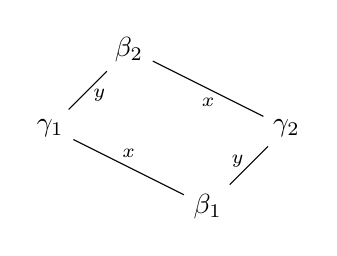
\begin{tikzpicture}[scale=1]
\draw
(0, 0) node(be2) {$\be_2$} 
(2,-1) node(ga2) {$\ga_2$}
(-1,-1) node(ga1){$\ga_1$}
(1,-2) node(be1) {$\be_1$}
(be2)
--node[pos=0.5, below]{$\ssty x$}
(ga2)
--node[pos=0.8, above]{$\ssty y$} 
(be1)
--node[pos=0.5, above]{$\ssty x$}
(ga1)
--node[pos=0.8, below]{$\ssty y$}
(be2);
\end{tikzpicture}
\qquad
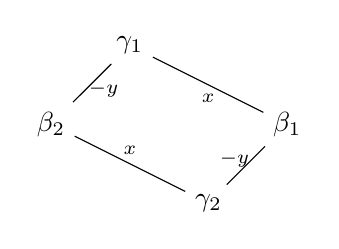
\begin{tikzpicture}[scale=1]
\draw
(0, 0) node(ga1) {$\ga_1$} 
(2,-1) node(be1) {$\be_1$}
(-1,-1) node(be2){$\be_2$}
(1,-2) node(ga2) {$\ga_2$}
(be2)
--node[pos=0.5, above]{$\ssty x$}
(ga2)
--node[pos=0.2, above]{$\ssty -y$} 
(be1)
--node[pos=0.5, below]{$\ssty x$}
(ga1)
--node[pos=0.2, below]{$\ssty -y$}
(be2);
\end{tikzpicture}
$$

(3)
We keep the notation of  part (2).
First, we assume that at least one of $\be_1$, $\be_2$, is long and prove that then $(\be_1, \be_2)=0$.
Let  $\be_1$ be long. 
Then, by Proposition~\ref{pro:summable-acute}~\ref{itm:long}, applied to the two pairs of summable roots $\be_1, -\ga_2$ and $\be_1, x$, we have $-(\be_1^\vee, \ga_2)=(\be_1^\vee, x)=-1$. 
Hence, $(\be_1^\vee, \be_2)=(\be_1^\vee, \ga_2+ x)=0$, which yields the claim.
The case $\be_2$ long is similar.
\par
Now, we assume $\be_1,\be_2\in \Phi_s$ and $(\be_1, \be_2)\neq 0$, and we prove that $|\ga_1|\neq |\ga_2|$.
Since $I$ is abelian, $\be_1$ and $\be_2$ are not summable, hence cannot have negative scalar product. 
Therefore $(\be_1, \be_2)> 0$, and since $|\be_1|=|\be_2|$,  by~\ref{sssec:general-roots}\ref{itm:length-ratio} we have $(\be_1^\vee, \be_2)=1$.  
By definition, we have $\be_2=\ga_1+y=\be_1+x+y$, hence 
$1=(\be_1^\vee, \be_2)=(\be_1^\vee, \be_1)+(\be_1^\vee, x)+(\be_1^\vee, y)=2+(\be_1^\vee, x)+(\be_1^\vee, y)$. 
It follows $(\be_1^\vee, x)+(\be_1^\vee, y)=-1$.
But, by Lemma~\ref{lem:corte-abeliani}\ref{itm:short-edge}, $x$ and $y$ are short, hence $(\be_1^\vee, x), (\be_1^\vee, y)\in \{0, \pm 1\}$  (by~\ref{sssec:general-roots}(2), again).
Therefore $\{(\be_1^\vee, x), (\be_1^\vee, y)\}=\{0, -1\}$.
We may assume $(\be_1^\vee, x)=0$ and $(\be_1^\vee, y)=-1$, without loss of generality.
Then, by Proposition~\ref{pro:summable-acute}(1), applied to the two summable pairs of short roots $\be_1, x$ and $\be_1, y$, we obtain $|\be_1|=|x|<|\be_1+x|=|\ga_1|$,  and $|\be_1|=|y|\geq |\be_1+y|=|\ga_2|$.  
Hence, $\ga_1$ is long and $\ga_2$ is short. 
\end{proof}
%\smallskip

\begin{ntn}
We write $\be_1< \{\ga_1, \ga_2\}< \be_2$ for  $\be_1< \ga_i<\be_2$ for both $i\in \{1, 2\}$.
\end{ntn} 
%\smallskip

Let $\{\be_1, \be_2\}$ and $\{\ga_1, \ga_2\}$ be crossing pairs. 
Up to exchange $\be_1$ and $\be_2$, we may assume $\be_2\not<\be_1$. 
Similarly, without loss of generality, we may assume $\ga_2\not< \ga_1$.
Then, by Proposition~\ref{pro:vert-comparable}\ref{itm:ordine}, either $\be_1< \{\ga_1, \ga_2\}< \be_2$, or $\ga_1< \{\be_1, \be_2\}< \ga_2$. 

\begin{defi}\label{def:lesssim}
We define the relations $\lesssim$ and $\sim$ on $\Phi^+$ as follows: 
\par
$\be_1\lesssim\be_2$
if and only if there exists $\ga_1, \ga_2\in \Phi^+$ such that 
 $\{\be_1, \be_2\}$ and $\{\ga_1, \ga_2\}$ are crossing pairs with $\be_1< \{\ga_1, \ga_2\}< \be_2$;
\par 
$\be_1\sim\be_2$
if and only if either $\be_1\lesssim \be_2$  or $\be_2\lesssim \be_1$.
\par
If  $\{\be_1, \be_2\}$ and $\{\ga_1, \ga_2\}$ are crossing pairs with $\be_1< \{\ga_1, \ga_2\}< \be_2$, we also say that $\{\ga_1, \ga_2\}$ is a {\it middle pair between} $\be_1$ and $\be_2$ and that $\{\be_1, \be_2\}$ is a {\it raising pair through} $\ga_1$ and $\ga_2$.
\end{defi}
%\smallskip

In the next corollary we study the order relations among different raising pairs through a common middle pair and  different middle pairs between a common raising pair. 

\begin{cor}\label{cor:catene-crossing}
Let $I$ be an abelian ideal, $\{\be_1, \be_2\}$ and $\{\ga_1, \ga_2\}$ be crossing pairs in $I$ with $\be_1< \{\ga_1, \ga_2\}< \be_2$. 
\begin{enumerate}
\item
If $\{\be'_1, \be'_2\}$ is any other raising pair through $\{\ga_1, \ga_2\}$, with $\be_1'<\be_2'$, then either $\be_1< \be'_1< \be'_2< \be_2$, or $\be'_1< \be_1< \be_2< \be'_2$. Moreover,  $\be_i-\be'_i\in \Phi$ for both $i=1, 2$.
\item
If $\{\ga'_1, \ga'_2\}$ is any other middle pair between $\{\be_1, \be_2\}$, then
$\ga_i-\ga'_j\in \Phi$ for all $i,j\in \{1, 2\}$. 
Moreover, one of the following four cases occur: $\ga'_i< \{\ga_1, \ga_2\}< \ga'_j$, $ \ga_i< \{\ga'_1, \ga'_2\}< \ga_j$ (with $\{i, j\}=\{1, 2\}$). 
In particular, there exists at most one incomparable middle pair between 
$\be_1$ and $\be_2$.
\end{enumerate}
\end{cor}

\begin{proof}
Under the assumption of (1), we have $\be_1'+\be_2'=\ga_1+\ga_2=\be_1+\be_2$, hence $\{\be'_1, \be'_2\}$ and $\{\be_1, \be_2\}$ are crossing pairs. 
Similarly, under the assumption of (2),  $\{\ga'_1, \ga'_2\}$ and $\{\ga_1, \ga_2\}$ are crossing pairs. Hence, the claim  follows directly from Proposition~\ref{pro:vert-comparable}\ref{itm:ordine}.  
\end{proof}

In the next lemma, we see that the possible lengths of roots and root differences in a crossing pair are very limited.

\begin{lem}\label{lem:lunghezze-radici-crossing}
Let $I$ be an abelian ideal in $\Phi^+$, $\{\be_1, \be_2\}$,  $\{\ga_1, \ga_2\}$ be crossing pairs contained in $I$, $\be_1 < \{\ga_1,\ga_2\} < \be_2$, 
$x=\be_2-\ga_2=\ga_1-\be_1$, and $y=\be_2-\ga_1=\ga_2-\be_1$.  
\begin{enumerate}
\item\label{itm:xy}
If either one of $x$, $y$ is long, then $x,y, \be_1$, $\be_2$, $\ga_1$, $\ga_2$ are all long. 
\item\label{itm:tutti}
If any one of $x$, $y$, $\be_1$, $\be_2$, $\ga_1$, $\ga_2$ is short,  then $x$ and $y$ are short and at most one of $\be_1$, $\be_2$, $\ga_1$, $\ga_2$ is long, except when $\ga_1=\ga_2$, in which case $\ga_1$ is short and $\be_1, \be_2$ are long. 
\end{enumerate}
\end{lem}

\begin{proof}
We first prove that:

(a) if any one of $\be_1$, $\be_2$, $\ga_1$, $\ga_2$ is short,  then $x$ and $y$ are short.
\par
We provide the details for the case $\ga_2\in \Phi_s$. 
The other cases are similar. 
We have $\ga_2+x=\be_2$, in particular $\ga_2+x\in I$, hence by Lemma~\ref{lem:corte-abeliani}\ref{itm:short-edge}, we obtain $x\in \Phi_s$.
Similarly, since $\ga_2+(-y)=\be_1\in I$ we obtain $-y\in \Phi_s$, hence the claim. 
\par
Now we prove that: 

(b) $x$ and $y$ are either both short, or both long.
\par
It suffices to prove that if either one of $x$, $y$ is short, then the other one is short, too.
Assume, for example, $x\in\Phi_s$. 
By (a), it suffices to prove that at least one among $\be_i,\ga_i\ (i=1,2)$, is short.
If $\be_1\in\Phi_s$, we are done.
Then, let $\be_1\in\Phi_\ell$. 
By Lemma~\ref{lem:esercizio}(3), the sum of two roots of different lengths is always short, hence  $\ga_1=\be_1+x$ is short and we are done.
The case $y\in\Phi_s$ is similar, hence (b) is proved.
\par
Now we conclude the proof of part (1). 
If either one of $x, y$ is long, then, by (a), $\be_i$ and $\ga_i$ are long, for $i=1,2$. 
Moreover, by (b), both of $x$ and $y$ are long. 

\par  
It remains to conclude the proof of part (2). 
So, we assume  $\{x, y, \be_1, \be_2, \ga_1, \ga_2\}\not\subseteq \Phi_\ell$.
Then, by part (1), $x, y\in \Phi_s$. 
We distinguish the two cases  $\ga_1\neq\ga_2$ and $\ga_1=\ga_2$.

\par
Let $\ga_1\neq\ga_2$. 
We have to prove that if any root in $\{\be_1, \be_2, \ga_1, \ga_2\}$ is long, then the  three remaining roots are short.

\par
Let $\be_1\in \Phi_\ell$.
By Lemma~\ref{lem:esercizio}(3) the sum of a long and a short root is short, hence we obtain $\ga_1, \ga_2\in \Phi_s$,  since $\ga_1=\be_1+x$ and  $\ga_2=\be_1+y$.
Then, we have $\ga_1, -x\in \Phi_s$, while $\ga_1+(-x)=\be_1\in \Phi_\ell$. By  Proposition~\ref{pro:summable-acute}(1), this implies $(\ga_1, -x)\geq 0$.

\par
If $\be_2\in \Phi_\ell$, arguing in a similar way, we obtain  
$\ga_1, \ga_2\in \Phi_s$. 
Moreover, $(\ga_1, y)\geq 0$.

\par
Now, if both $\be_1, \be_2\in \Phi_\ell$, we deduce $(\ga_1^\vee, \ga_2)=(\ga_1^\vee, \ga_1-x+y)\geq (\ga_1^\vee, \ga_1)=2$. 
Since $|\ga_1|=|\ga_2|$,  by~\ref{sssec:general-roots}(2) this implies $\ga_1=\ga_2$, contrary to the assumption.

\par
By a similar argument, taking into account that $\be_1\neq \be_2$, we obtain that if one of $\ga_1$, $\ga_2$ is long, the three remaining roots in the crossing pairs are short, as claimed.

\par 
Now, let $\ga_1=\ga_2$. 
We have to prove that $\ga_1\in \Phi_s$ and $\{\be_1, \be_2\}\subseteq\Phi_\ell$.
Indeed, we have $\be_1+\be_2=2\ga_1$, hence $(\be_1+\be_2, \ga_1^\vee)=4$. 
By~\ref{sssec:general-roots}(2), it follows that either $(\be_1,\ga_1^\vee)=(\be_2,\ga_1^\vee)=2$,
or $(\be_1,\ga_1^\vee)=1$ and $(\be_2,\ga_1^\vee)=3$. 
In the first case we obtain $\ga_1\in \Phi_s$ and $\be_1, \be_2\in \Phi_\ell$, as claimed.
The latter case cannot happen, otherwise we obtain $s_{\ga_1}(-\be_2)=-\be_2+3\ga_1\in \Phi$, and $-\be_2+3\ga_1=(-\be_2+2\ga_1)+\ga_1=\be_1+\ga_1$, contrary to abelianity of $I$.
\end{proof}

In the next proposition, we prove that, for any pair of comparable roots $\be_1$ and $\be_2$ in an abelian ideal $I$, if $\be_1-\be_2$ is  not a root, then $\be_1\sim \be_2$. 
Moreover, we analyze when the reverse implication holds. 
We need the following well known result. 

\begin{lem}[{\cite[Ch.~VI, \S~1.9, Proposition~19]{Bou}}]\label{lem:somme-bou}
Let $\ga_1,\dots, \ga_m\in \Phi^+$. 
If  $\ga_1+\cdots+\ga_m\in \Phi^+$, 
there exists a permutation $(\ga'_1, \dots, \ga'_m)$ of $(\ga_1, \dots,\ga_m)$ such that $\ga'_{1}+\cdots+\ga'_{h}\in \Phi$ for all $h\in\{1, \dots, m\}$. 
\end{lem}

\begin{pro}\label{pro:minori-crossing}
Let $I$ be an abelian ideal in $\Phi^+$ and $\be_1, \be_2\in I$. 
\begin{enumerate}
\item 
If $\be_1<\be_2$ and $\be_2-\be_1\not\in\Phi$, then $\be_1\lesssim\be_2$.
\label{itm:nonroot-then-sim}
\item 
If $\be_1\lesssim\be_2$, $\{\be_1, \be_2\}\subseteq\Phi_s$ and there exists a middle pair $\{\ga_1, \ga_2\}$ between $\be_1, \be_2$ such that $\ga_1\in\Phi_s$ and $\ga_2\in\Phi_\ell$, then $\be_2-\be_1\in\Phi_s$.
\label{itm:sim-then-root}
\item
If $\be_1\lesssim\be_2$, then  $\be_2-\be_1\not\in\Phi$ if and only if either one of the following conditions is satisfied:
\begin{enumerate}[label=\textup{(\alph*)}]
\item at least one of $\be_1$, $\be_2$ is long,
\item $\{\be_1, \be_2\}\subseteq\Phi_s$ and there exists  a middle pair $\{\ga_1, \ga_2\}\subseteq\Phi_s$ between $\be_1, \be_2$.
\end{enumerate}
\label{itm:sim-then-nonroot}
\end{enumerate}
\end{pro}


\begin{proof}
(1) Let $\be_1< \be_2$ and $\be_2-\be_1\not\in\Phi$. By definition, $\be_2-\be_1$ is a sum of positive roots. Let 
$$
k=\min\{h\in \nat \mid \exists\, \eta_1,\dots, \eta_h\in \Phi^+ \text{ such that }  \be_2-\be_1=\eta_1+\cdots+\eta_h\},
$$ 
and $\eta_1,\dots, \eta_k\in \Phi^+$ be such that $\be_2=\be_1+\eta_1+\cdots+\eta_k$. 
By assumption, $k\geq 2$. 
Moreover, by minimality of $k$, no partial sum $\sum_{j=1}^h\eta_{i_j}$ with $1\leq i_j\leq k$ and $h> 1$  is a root.
\par
By Lemma~\ref{lem:somme-bou},  we may find a permutation $(\ga'_1, \dots, \ga'_m)$ of the sequence $(\be_1, \eta_1, \dots,$ $\eta_n)$ such that all partial sums $\ga'_1+\cdots+\ga'_h$ are roots.
By the above discussion,  $\be_1$ must be either $\ga'_1$, or $\ga'_2$.
In both cases, we easily obtain that there exists a permutation $(\eta'_1, \dots, \eta'_k)$ of $(\eta_1, \dots, \eta_k)$ such that $\be_1+\sum\limits_{1\leq j\leq h}\eta'_j\in \Phi$ for all $h\in \{0, \dots, k\}$.
\par
Now, we prove that also $\be_2-\eta'_1=\be_1+\sum\limits_{2\leq j\leq k}\eta'_j\in \Phi$. 
This yields the crossing relation  $\be_1+\be_2=(\be_1+\eta'_1)+(\be_2-\eta'_1)$, which concludes the proof of (1). 
\par
Let $\ga_h=\be_1+\sum\limits_{1\leq j\leq h}\eta'_j$,
so that $\ga_k=\be_2$. 
We prove, by induction on $h$, that $\ga_h-\eta_1\in \Phi$ for all $h\in \{1, \dots, k\}$. 
For $h=1$, the claim is clear, since $\ga_1=\be_1+\eta'_1$, by definition.
Assume $1\leq h<k$ and   $\ga_h-\eta'_1\in \Phi$. 
We have 
$$
\ga_{h+1}=\ga_h+\eta'_{h+1}=(\ga_h-\eta'_1)+\eta'_1+\eta'_{h+1}.
$$
By our assumption, $\eta'_1+\eta_{h+1}'\not\in \Phi$, hence, by  Proposition~\ref{pro:smart}, applied to the summable triad $(\ga_h-\eta'_1), \eta'_1, \eta'_{h+1}$, we obtain that $(\ga_h-\eta'_1)+\eta'_{h+1}$ is a root (and also $(\ga_h-\eta'_1)+ \eta'_1$ is a root).
Since $(\ga_h-\eta'_1)+\eta'_{h+1}=\ga'_{h+1}-\eta'_1$, we get the claim.
%\smallskip

(2)  Let $\be_1+\be_2=\ga_1+\ga_2$, \ $\be_1< \{\ga_1, \ga_2\}< \be_2$, \ $\be_1, \be_2, \ga_1\in \Phi_s$,  and  $\ga_2\in \Phi_\ell$. 
We have to prove that $\be_2-\be_1\in \Phi_s$.  
First, we see that the condition $(\be_2, \be_1^\vee)>0$ implies the claim.
Indeed, by~\ref{sssec:general-roots}(1) if $(\be_2, \be_1^\vee)>0$, then $\be_2-\be_1\in \Phi$.  
Moreover, $\be_2-\be_1\not\in \Phi_\ell$, otherwise, by Proposition~\ref{pro:summable-acute}~\ref{itm:general}, we should have $(\be_2, -\be_1^\vee)\geq 0$.
\par
Thus, we prove that $(\be_2, \be_1^\vee)>0$.
Let $x=\be_2-\ga_2=\ga_1-\be_1$. 
We recall that $x$ is short, by Lemma~\ref{lem:lunghezze-radici-crossing}~\ref{itm:xy}. 
Then, $(\be_2, \be_1^\vee)=(\ga_2, \be_1^\vee)+(x, \be_1^\vee)$, and our assumptions on lengths imply $(x, \be_1^\vee)\in \{0, \pm 1\}$ and $(\ga_2, \be_1^\vee)\in \{0, \pm2, \pm 3\}$, by~\ref{sssec:general-roots}(2).
Moreover, $(\ga_2, \be_1^\vee)$ is positive, by Proposition~\ref{pro:vert-comparable}\ref{itm:edges-are-roots}, hence,  $(\ga_2, \be_1^\vee)\geq 2$ and $(\be_2, \be_1^\vee)\geq 2-1=1$, as claimed.
%\smallskip

(3)
For proving the \lq\lq if\rq\rq\ part, it suffices to prove that if neither (a), nor (b) hold, then the assumption of (2) holds.
First, we assume that (a) does not hold, i.e., $\be_1, \be_2\in \Phi_s$. 
Then, by Lemma~\ref{lem:lunghezze-radici-crossing}~\ref{itm:tutti}, for all middle pairs $\{\ga_1, \ga_2\}$ between $\be_1, \be_2$, at most one of $\ga_1, \ga_2$ is long.
It follows that either (b) holds, or all middle pairs $\{\ga_1, \ga_2\}$ satisfies the assumption in (2).

\par
It remains to prove the \lq\lq only if\rq\rq\ part. 
Let  $\ga_1, \ga_2\in \Phi$ be such that $\be_1+\be_2=\ga_1+\ga_2$ and $\be_1< \{\ga_1, \ga_2\}< \be_2$.
\par
(a) Assume $\be_2\in \Phi_\ell$ and, as before, let $x=\ga_1-\be_1=\be_2-\ga_2$ and $y=\ga_2-\be_1=\be_2-\ga_1$. 
Since the pairs of $\be_2, -x$ and $\be_2, -y$ are summable,  by Proposition~\ref{pro:summable-acute}(2) we obtain $(x, \be_2^\vee)=(y, \be_2^\vee)=1$.
Hence,
$$
2=(\be_2, \be_2^\vee)=(\be_1+x+y, \be_2^\vee)=(\be_1, \be_2^\vee)+2.
\leqno({*)}
$$
It follows $(\be_1, \be_2^\vee)=0$ and, by Proposition~\ref{pro:summable-acute}(2), $\be_2-\be_1\not\in \Phi$.
If $\be_1\in \Phi_\ell$, we may argue in a similar way and find again $\be_2-\be_1\not\in \Phi$.  
\par
(b) Let $\be_1, \be_2\in \Phi_s$.
By Proposition~\ref{lem:lunghezze-radici-crossing}~\ref{itm:xy}, we have $x,y\in \Phi_s$, hence, by applying Lemma~\ref{lem:esercizio}~\ref{itm:all-equal-lengths} to the summable pairs $\be_2, -x$ and $\be_2, -y$, we obtain that  equalities  ($*$) still hold. 
Hence, also in this case we have $\be_2-\be_1\not\in \Phi$.
\end{proof}
%\smallskip

The following corollary follows directly from parts~\ref{itm:nonroot-then-sim} and~\ref{itm:sim-then-nonroot} of Proposition~\ref{pro:minori-crossing}.

\begin{cor}\label{cor:minori-crossing}
Let $I$ be an abelian ideal in $\Phi^+$, and $\be_1, \be_2\in I$.
If either one of $\be_1$, $\be_2$ is long, then $\be_1\lesssim \be_2$ if and only if $\be_1< \be_2$ and  $\be_2-\be_1\not\in \Phi$. 
\end{cor}

If we combine parts \ref{itm:sim-then-root} and \ref{itm:sim-then-nonroot} of Proposition~\ref{pro:minori-crossing}, we obtain that the root lengths of all middle pairs between two fixed short roots $\be_1, \be_2$ are uniquely determined by $\be_1, \be_2$.

\begin{cor}\label{cor:minori-crossing-2}
Let $I$ be an abelian ideal in $\Phi^+$, $\be_1, \be_2\in I\cap \Phi_s$, and $\be_1\lesssim \be_2$.
Then either $\ga_1, \ga_2\in \Phi_s$ for all middle pairs  $\{\ga_1, \ga_2\}$ between $\be_1, \be_2$, 
or $\ga_1$ and $\ga_2$ have different lengths for all middle pairs  $\{\ga_1, \ga_2\}$ between $\be_1, \be_2$.
\end{cor}

\begin{proof}
Let $\{\ga_1, \ga_2\}$ and $\{\ga'_1, \ga'_2\}$ be middle pairs between $\be_1, \be_2$. 
By Proposition~\ref{lem:lunghezze-radici-crossing}\ref{itm:sim-then-root}, at least one of $\ga_1, \ga_2$ and at least one of $\ga'_1, \ga'_2$ are short.
If $\{\ga_1, \ga_2\}\not\subseteq \Phi_s$ then, by part \ref{itm:sim-then-root} of Proposition~\ref{pro:minori-crossing}, we have $\be_2-\be_1\in \Phi_s$, while if $\{\ga'_1, \ga'_2\}\subseteq \Phi_s$, then, by part \ref{itm:sim-then-nonroot} we have $\be_2-\be_1\not\in \Phi$.
Hence the two possibilities mutually exclude each other.
\end{proof}

\begin{defi}\label{def:red}
For any  $S\subseteq\Phi^+$,  
we say that $S$ is reduced if, for all $\be, \be'\in S$, $\be\nosim \be'$. 
\par
For all $\be\in \Phi^+$ we set 
$$
\red(\be)=\{\be'\in \Phi^+\mid \be\neq \be' \text{ and } \be\not\sim \be'\}.
$$
\end{defi}
%\smallskip

\begin{rem}\label{rem:red}
By Proposition~\ref{pro:minori-crossing}\ref{itm:nonroot-then-sim} and Lemma~\ref{lem:corte-abeliani}\ref{itm:non-ortogonali}, if $I$ is an abelian ideal, $\be\in I$, and $I( \be^{\comp})=\{\ga\in I\mid \ga\text{ is comparable with }\be\}$, then 
\begin{equation}\label{eq:red}
\red(\be)\cap I( \be^{\comp})\subseteq \{\ga\in I \mid \ga-\be\in \Phi^+\}= \{\ga\in I\smeno\{\be\}\mid (\ga,\be)> 0\}.
\end{equation}
If $\be\in \Phi_\ell$, in particular in the simply laced case, the inclusion is an equality, by Corollary~\ref{cor:minori-crossing}. 
Moreover, if $\be\in \Phi_\ell$, we have $(\ga, \be^\vee)\in \{0, \pm 1\}$ for all $\ga\in \Phi\smeno\{\be\}$, hence 
\begin{equation}\label{eq:red-2}
\red(\be)\cap I( \be^{\comp}) =\{\ga\in I \mid (\ga,\be^\vee) = 1\}.
\end{equation}
In general, the inclusion in \eqref{eq:red} is proper. 
As an example, for $\Phi$ of type $\mathrm C_n$, if we number the simple roots as in \cite{Bou} and take $I=(\al_n^\leq)$,  $\be_1=\al_n+\al_{n-1}, \be_2=\al_n+2\al_{n-1}+\al_{n-2}, \ga_1=\al_n+\al_{n-1}+\al_{n-2}, \ga_2=\al_n+2\al_{n-1}$, we have: $\be_1+\be_2=\ga_1+\ga_2$, hence $\be_1\lesssim \be_2$, but $\be_2-\be_1=\al_{n-1}+\al_{n-2}\in \Phi_s$.
This is an example of case~\ref{itm:sim-then-root} of Proposition~\ref{pro:minori-crossing}.
\end{rem}



\section{Triangulation orders}\label{sec:triang-order} 

In this section we define some special orderings of abelian ideals, which we call triangulation orders, and prove that all facet ideals have a triangulation order.
Throughout the section, let $I$ be an abelian ideal of $\Phi^+$ such that $\rk(I)=n$.
By \lq\lq hyperplane\rq\rq, we mean  \lq\lq linear hyperplane\rq\rq.

\pagebreak


\begin{defi}\label{def:bipartite}
Let $J \subseteq I$.
We say that $J$ is {\it bipartite} if it has an initial section  $J_{\mathrm i}$, and a final section $J_{\mathrm f}$ such that 
\begin{enumerate}
\item $J=J_{\mathrm i}\cup J_{\mathrm f}$; 
\item for all $\be_1\in J_{\mathrm i}\smeno J_{\mathrm f}$  and $\be_2\in J_{\mathrm f}\smeno J_{\mathrm i}$, we have  $\be_1\lesssim \be_2$;
\item there exists a hyperplane $H$ in $\mathrm E$ such that $J_{\mathrm i}\cap J_{\mathrm f}\subseteq H$ and $H$ strictly separates  $J_{\mathrm i}\smeno J_{\mathrm f}$  from~$J_{\mathrm i}\smeno J_{\mathrm f}$.
\end{enumerate}
If the above conditions hold, we say that $\{J_{\mathrm i},J_{\mathrm f}\}$ is a  {\it bipartition} of $J$.
If, moreover, both $J_{\mathrm i}$ and  $J_{\mathrm f}$ are proper subsets of $J$, we say that $\{J_{\mathrm i},J_{\mathrm f}\}$ is a {\it proper} bipartition.  
A hyperplane $H$ as in (3) is called a {\it separating hyperplane}, for the bipartition  $\{J_{\mathrm i},J_{\mathrm f}\}$ of $J$.
\end{defi}

Note that, by definition, if $J$ has a proper bipartition, then  it has at least two elements. 
If $J$ is also saturated, then it contains two crossing pairs and these provide at least three elements in $J$.
The definition also implies that, if  $\{J_{\mathrm i}, J_{\mathrm f}\}$ is a  bipartition of $J$, then $J_{\mathrm i}\smeno J_{\mathrm f}$ and $J_{\mathrm f}\smeno J_{\mathrm i}$ are an initial and a final section of $J$, respectively, 
since the complement of an initial section is a final section, and vice-versa, and we have $J=(J_{\mathrm i}\smeno J_{\mathrm f})\sqcup J_{\mathrm f}=J_{\mathrm i}\sqcup (J_{\mathrm f}\smeno J_{\mathrm i})$, where by $\sqcup$ we denote disjoint union. 
Finally, we note that if $J$ is saturated, also all the subsets $J_{\mathrm i}$, $J_{\mathrm f}$,  $J_{\mathrm i}\smeno J_{\mathrm f}$, $J_{\mathrm f}\smeno J_{\mathrm i}$, and $J_{\mathrm i}\cap  J_{\mathrm f}$ are saturated. 

%\smallskip

\begin{defi} \label{def:restricted-sim}
For each subset  $S$ of $\Phi^+$, we define the restricted relations $\lesssim_S$ and $\sim_S$ on $S$ as follows.
For all $\be_1, \be_2\in S$ we set: \upn{(1)} $\be_1 \lesssim_S \be_2$ if there exists a middle pair $\{\ga_1, \ga_2\}$ between $\be_1$ and $\be_2$ contained in $S$; 
\upn{(2)} $\be_1 \sim_S \be_2$  if either $\be_1 \lesssim_S \be_2$, or $\be_2 \lesssim_S \be_1$.
We say that $S$ is  $\sim$closed if, for all $\be_1, \be_2\in S\cap \Phi^+$,   $\be_1 \lesssim\be_2$ implies   $\be_1 \lesssim_S  \be_2$. 
\end{defi}

Obviously, for any $S\subseteq \Phi^+$ and $\be_1, \be_2\in S$, the relation $\be_1 \lesssim_S \be_2$ implies $\be_1 \lesssim \be_2$.
Hence, if $S$ is~$\sim$closed, then, for all  $\be_1, \be_2\in S$, we have $\be_1\sim\be_2$ if and only if $\be_1\sim_S\be_2$.

The first of following lemmas is clear, hence we omit the proof.

\begin{lem}\label{lem:saturated-are-simclosed}
Let $S\subseteq \Phi^+$. 
If $S$ is saturated, then $S$ is $\sim$closed.
\end{lem}

\begin{lem}\label{lem:reduced-component-wise}
Let I be an abelian ideal in $\Phi$, $\Psi$ a root subsystem of $\Phi$, and $\Psi_1, \dots, \Psi_k$ be the irreducible components of $\Psi$. 
Moreover, let $J$ be a $\sim$closed subset of $\Phi$ such that $J\subseteq I\cap \Psi$, and  let $R\subseteq J$.
Then, $R$ is reduced in $\Phi$ if and only if $R\cap \Psi_i$ is reduced in $\Psi_i$ for all $i\in \{i, \dots, k\}$.
\end{lem}

\begin{proof}
The \lq\lq only if\rq\rq\ part is obviuos. 
Conversely, we assume that $R\cap \Psi_i$ is reduced in $\Psi_i$ for all $i\in \{i, \dots, k\}$ and prove that $R$ is reduced in $\Phi$.
By contradiction, let $\be_1\lesssim \be_2$ for some $\be_1, \be_2\in R$. 
Then, since $J$ is $\sim$closed, there exists a middle pair $\{\ga_1, \ga_2\}$, between $\be_1$ and $\be_2$, contained in $J$, hence in $\Psi$. 
By Proposition~\ref{pro:vert-comparable}\ref{itm:edges-are-roots}, $(\be_j,\ga_{j'})>0$  for all $j,j'\in \{1, 2\}$, hence,  there exists $i\in \{1, \dots, k\}$ such that $\be_j,\ga_j\in \Psi_i$, for all $j\in \{1, 2\}$. 
Thus, we have $\be_1\lesssim_{\Psi_i}\be_2$, contrary to the assumption.
\end{proof}

\begin{lem}\label{lem:simclosed-suff-cond}
Let $I$ be an abelian nilradical of $\Phi^+$, $\Psi$ a parabolic root subsystem of $\Phi$, and $\Pi_\Psi$ the simple system of $\Psi^+$.
Assume that the following conditions hold:  
\begin{enumerate}[label=\textup{(\alph*)}]
\item $\Pi_\Psi\smeno I\subseteq \Pi$; 
\item if $\Psi'$, $\Psi''$ are distinct irreducible components of $\Psi$, then $I\cap\Psi'$ and  $I\cap \Psi''$ are element-wise incomparable.
\end{enumerate} 
Then $I\cap \Psi$ is saturated,  hence $\sim$closed. 
\end{lem}

\begin{proof}
Let $\ga_1, \ga_2\in I\cap \Psi$ with $\ga_1< \ga_2$.
Then   $\ga_2-\ga_1$ is a linear combination of roots in $\Pi$ with non-negative, integral, coefficients. 

\par
Let $\Psi_1, \dots, \Psi_k$ be the irreducible components of $\Psi$ and $\Pi_{\Psi_i}$ the simple system of $\Psi_i$, for $i=1, \dots, k$. 
By assumption (b), there exists $i\in \{1, \dots, k\}$ such that $\ga_1, \ga_2\in \Psi_i$. 

\par
By Proposition~\ref{pro:induzione-fine}, $I\cap \Psi_i\neq\emptyset$ if and only if there exists $\be_i^*\in I\cap \Pi_{\Psi_i}$. 
Moreover, in such a case, we have $I\cap \Pi_{\Psi_i}=\{\be_i^*\}$, and $I\cap \Psi_i=\Psi_i^+\smeno\Phi(\Pi_{\Psi_i}\smeno\{\be_i^*\})$.
It follows that $\ga_2-\ga_1$ is a $\ganz$-linear combination of roots in $\Pi_{\Psi_i}\smeno {\be_i^*}$. 

\par
By assumption (a), $\Pi_{\Psi_i}\smeno {\be_i^*}\subseteq \Pi$, hence, being $\Pi$ a linear basis of $E$, $\ga_2-\ga_1$ is a linear combination of roots in $\Pi_{\Psi_i}\smeno {\be_i^*}$ with non-negative integral coefficients. 
Since $\Psi$, and hence $\Psi_i$, is parabolic, we obtain that all $\ga\in \Phi$ such that $\ga_1\leq \ga\leq \ga_2$ belong to $\Psi_i$, hence to  $I\cap\Psi_i$. 

\par
This proves that $I\cap \Psi$ is saturated and hence, 
by Lemma~\ref{lem:saturated-are-simclosed}, also $\sim$closed.
\end{proof}

We recall that we have defined the set $\red(\be)$, for  $\be\in \Phi^+$,  in  Definition~\ref{def:red}.

\begin{defi}\label{def:detachable}
Let $J\subseteq I$, and $\be\in J$.
We say that $\be$ is a {\it detachable} element in $J$ if the following conditions hold:
\begin{enumerate}
\item
$\be$ is an extremal element of $J$ \upn(with respect to the standard partial order\upn); 
\label{itm:extremal}
\item there exists a hyperplane $H$ such that:
\begin{enumerate}[label=\textup{(\alph*)}]
\item  $J\cap \red(\be)=J\cap H$ and $H$ strictly separates $\be$ from $J\smeno(\{\be\}\cup \red(\be))$;
\label{itm:separa}
\item
$I\cap H $ is  $\sim$closed.
\label{itm:chiuso} 
\end{enumerate}
\label{itm:hyperplane}
We call such a hyperplane $H$ a {\it detaching hyperplane} for $\be$ in $J$.
\end{enumerate}
\end{defi}


\begin{lem}\label{lem:detachable}
Let $I$ be a facet ideal, $\be\in I\cap \Phi_\ell$, and $I(\be^{\comp})=\{\ga\in I\mid \ga\leq\be\text{ or } \be\leq \ga\}.$ 
Then, there exists a hyperplane $H$ such that $I\cap H$ is~$\sim$closed  and $I(\be^{\comp})\cap \red(\be)=I\cap H$.
\par
Moreover, if $J$ is such that $J\subseteq I(\be^{\comp})$, and $\be$ is an extremal element of $J$, then $H$ is a detaching hyperplane for $\be$ in $J$.
\end{lem}

\begin{proof}
By Remark~\ref{rem:red}, $I(\be^{\comp})\cap \red(\be)=\{\ga\in I \mid (\ga, \be^\vee)=1\}$.
Let $\al_I$ be the (unique) simple root such that $I=\{\ga\in \Phi\mid c_{\al_I}(\ga)=m_{\al_I}\}$. 
Recall that $\check\omega_{\al_I}$ is the fundamental coweight such that $(\al_I, \check\omega_{\al_I})=1$ and $(\al, \check\omega_{\al_I})=0$ for all $\al\in \Pi\smeno \{\al_I\}$.
We set \ $\nu=m_{\al_I}\be^\vee-\check\omega_{\al_I}$ \ and \ $H=\nu^\perp$.
Then, for all $\ga\in I$,  we have $(\nu, \ga)=0$ if and only if $(\be^\vee, \ga)=1$, hence $I\cap H= I(\be^{\comp})\cap \red(\be)$.

\par 
Now, we prove that $I\cap H$ is $\sim$closed. 
Let $\be_1, \be_2\in \Phi^+\cap H$, $\be_1\sim\be_2$, and $\{\ga_1,\ga_2\}$ be a middle pair between $\be_1$ and $\be_2$.
Then $(\ga_1+\ga_2, \be^\vee)=(\be_1+\be_2, \be^\vee)=2$. 
Since $\be$ is long, this forces $(\ga_1, \be^\vee)=(\ga_2, \be^\vee)=1$, hence $\{\ga_1,\ga_2\}\subseteq I \cap H$, which implies the claim.

\par
It remains to prove the second assertion.
Let $J\subseteq I(\be^{\comp})$ and $\be$ be an extremal element in $J$.
Then, by  the previous part, $J\cap \red(\be)= J\cap H$.
In order to prove that $H$ is a detaching hyperplane for $\be$ in $J$, it remains to prove that $H$ strictly  separates $\be$ from $J\smeno (\{\be\}\cup H)$.
We prove that $H$ strictly  separates $\be$ from $I\smeno (\{\be\}\cup H)$, which implies the claim.
Since $I$ is abelian, we have $(\be^\vee, \ga)\geq 0$ for all $\ga\in I$.
Moreover, we have $(\be^\vee, \ga)\in \{0, \pm 1\}$, since $\be\in \Phi_\ell$.
Therefore, for all $\ga\in I\smeno H$,  we have $(\be^\vee, \ga)=0$, hence  $(\nu, \ga)=-m_{\al_I}$.
Moreover,  we have $(\be, \nu)=m_{\al_I}$, hence the claim is proved.
\end{proof}

\begin{defi}\label{def:triang-order}
Let 
$\preccurlyeq$ be a total order relation on $I$,  and 
$$
S_{I,\preq}=\{\be\in I\mid \rk(\be^\preq)=n\}.
$$ 
We say that $\preq$ is {\em a triangulation order} if the following conditions hold:
\begin{enumerate}
\item\label{itm:interno}
$I\smeno S_{I,\preq}$ is saturated; 
\item\label{itm:esterno}
for each $\be\in S_{I,\preq}$,  $(\be^\preq)$ is saturated and either one of the following conditions holds:
\begin{enumerate}[label=\textup{(\alph*)}]
\item $\be$ is detachable in  $(\be^\preq)$,  
\item $(\be^\preq)$ has a bipartition $\{J_{\mathrm i}, J_{\mathrm f}\}$ such that,  for both $J=J_{\mathrm i}$ and $J=J_{\mathrm f}$, $\be$ is detachable in $J$.%, and there exists a detaching hyperplane $H_J$, for $\be$ in $J$, such that $(\be^\preq) \cap H_J\subseteq \red(\be)$.
\end{enumerate}
\end{enumerate}
\end{defi}

\begin{rem}\label{rem:ini-sec}~\\[-1em]
\begin{enumerate}
\item
The definition directly implies that, for any total ordering $\preq$  on $I$, the subset $S_{I,\preq}$ is an initial section of the ordered set $(I, \preq)$.
Moreover, we have $\rk(I\smeno S_{I,\preq})< n$.
\item 
The set $I\smeno S_{I,\preq}$ may be properly contained in $I\cap \gen(I\smeno S_{I,\preq})$. 
For the triangulation orders that we will construct, this
happens exactly in one case, namely for type $\mathrm E_{7}$.
\item
The above definition does not contain any condition on the restriction of $\preq$ to $I\smeno S_{I,\preq}$. 
Hence, if $\preq$ is a triangulation order, any other total order $\preq'$ such that  $S_{I,\preq'}=S_{I,\preq}$, and  $\preq$ and $\preq'$ coincide on the initial section $S_{I,\preq}$, is a triangulation order, too.
\end{enumerate}
\end{rem}

We will prove the existence of triangulation orders for all facet ideals.  
The proof requires a case by case analysis. 
By Proposition~\ref{pro:faces-are-abnil}, we may restrict the analysis to the abelian nilradicals.

\begin{defi}
We say that the facet ideal $I$ of $\Phi^+$  is an abelian nilradical of type $\mathrm X_{n,k}$, and we write $I\cong \mathrm X_{n,k}$, if there exists an irreducible root subsystem $\Psi$ of $\Phi$ and a positive system $\wt \Psi^+$ of $\Psi$ such that: 
\begin{enumerate}
\item
$I$ is an abelian nilradical of $\wt \Psi^+$;
\item 
$\Psi$ is of type $\mathrm X_n$; 
\item 
if $\{\al'_1, \dots, \al'_n\}$ is a simple system of $\wt \Psi^+$, numbered according to Bourbaki's conventions \cite{Bou}, then $I$ is the principal ideal generated by $\al'_k$ in $\wt \Psi^+$.
\end{enumerate}
\end{defi}

It is implicit in the definition that the above $\al'_k$ has multiplicity $1$ in $\Psi$. 

\par
We note that the type of a facet ideal may be not unique, if the root system $\Psi$ has nontrivial Dynkin diagram automorphisms. 
We identify the types $\mathrm X_{n,k}$ and $\mathrm X_{n,k'}$ if there exists a diagram automorphism that maps $\al_k$ into $\al_{k'}$.   
By a direct inspection of the highest root in all root types, we see that the possible abelian nilradicals types,  in an irreducible root system of rank $n$, are the following:  
$$
\mathrm A_{n, k}\ \text{ for } k=1,\dots, n, \xuad \mathrm B_{n,1},\xuad \mathrm C_{n, n},\xuad \mathrm D_{n,k}\ \text{ for } k=1, n-1, n,\xuad \mathrm E_{6,1},\xuad  \mathrm E_{6,6},\xuad \mathrm E_{7, 7}.
$$
Among them, we have  the identifications: $\mathrm A_{n, k}=\mathrm A_{n, k'}$
for $k+k'=n+1$; $\mathrm D_{n,n-1}=\mathrm D_{n,n}$ for all $n\geq 4$ and  $\mathrm D_{4,1}=\mathrm D_{4,3}=\mathrm D_{4,4}$; $\mathrm E_{6,1}=\mathrm E_{6,6}$.

\par
By  Proposition~\ref{pro:faces-are-abnil},  the facet ideals that are not abelian nilradicals of $\Phi^+$ are in any case abelian nilradicals of some type. 
Their type  $\mathrm X_{n,k}$ is explicitly obtained as follows.

\par
If the type of $\Phi$ is $\mathrm A_n$, all the facet ideals are nilradicals of $\Phi^+$, hence we may assume that the extended Dynkin graph of $\Phi$ is a tree.
Then, $I_{\mathrm F_{\al_i}}$ is a facet ideal of $\Phi^+$ if and only if  $\al_i$ is a leaf in the extended Dynkin graph.
By Corollary~\ref{cor:proIMRN}, the Dynkin graph obtained by removing $\al_i$ from the extended Dynkin graph of $\Phi$, gives the root type $\mathrm X_n$. 
Moreover, the position of $-\theta$ in the new Dynkin graph gives the index $k$ of the abelian nilradical type $\mathrm X_{n,k}$. 
Below, we write the resulting type for the facet ideals that are not abelian nilradicals of $\Phi^+$ itself. 
If the root type of $\Phi$ is  $\mathrm Y_n$, we write $I_F(\mathrm Y_n, \al_i)$ in place of $I_{F_{\al_i}}$.
\begin{align*}
&I_F(\mathrm B_n,\al_n)\cong \mathrm D_{n,n},\qquad 
I_F(\mathrm F_4,\al_4)\cong \mathrm B_{4,1},\qquad 
I_F(\mathrm E_7,\al_2) \cong \mathrm A_{7,1},
\\ 
&I_F({\mathrm E_8},\al_1)\cong \mathrm D_{8,1},\qquad I_F(\mathrm E_8,\al_2) \cong \mathrm A_{8,1}.
\end{align*}

\par
In proving the next proposition, we will consider, case by case, the seven possible distinct sporadic or classes of abelian nilradical types.  
The main points of the proof are illustrated in Figures 1--9. 
We first give some explanation of these figures. 
We may arrange the roots of any facet ideal $I$ in a matrix $(\be_{i,j})$, in such a way that adjacent entries differ by a simple root. 
The label $i$ on a certain edge means that  the difference between its vertexes is the simple root $\al_i$. 
We choose the matrix arrangement of roots so that the standard partial order is compatible with the reverse lexicographic order of row and column indexes, starting from $\be_{1,1}=\theta$.
In this way, the matrix yields a Hasse diagram of $I$ in which  the order ascends toward northwest. 
We note that this condition does not determine a unique possibility. 
The figures illustrate  the proof on such Hasse diagrams for all the abelian nilradicals.

\begin{pro}\label{pro:tri-ord-existence}
Each facet ideal has a triangulation order.
\end{pro}

\begin{proof}
By the above discussion, we may assume that $I$ is an abelian nilradical of~$\Phi^+$. 
\par
By Remark~\ref{rem:ini-sec}, it suffices to define a subset $S_{I,\preq}$  of $I$ and a partial order $\preq$ on $I$ that is total on $S_{I,\preq}$ and has $S_{I,\preq}$ as an initial section, in such a way that all conditions of Definition~\ref{def:triang-order} are satisfied. (In figures 1-9, the circled nodes correspond to the elements in $S_{I,\preq}$.)
\par
Henceforward, we write $S_I$ in place of $S_{I,\preq}$ and we intend that $S_I$ is an initial section of~$\preq$.
We will define the restriction $(S_I, \preq)$ as a sequence $(\be_1, \dots, \be_k)$ (so that $(\be_i^\preq)=\{\be_i, \dots, \be_k\}\cup (I\smeno S_I)$).
Then, we will find a hyperplane $H_I$ such that $\gen(I\smeno S_I)=H_I$ and $\be_k\not\in H_I$: this ensures that  $S_I$ is well defined, i.e. $S_I=\{\be\in I\mid \rk(\be^\preq)=n\}$.
Moreover, we will prove that $I\smeno S_I$ is saturated (condition~\ref{itm:interno} of Definition~\ref{def:triang-order}). 
\par
In all cases, the sequence $(\be_1, \dots, \be_k)$ will be such that,  for $i=1, \dots, k$,  $\be_i$ is extremal in $(\be_i^\preq)$, with respect to the standard partial order. 
Since $I\smeno S_I$ is saturated, this implies that  $(\be_k^\preq)$ is saturated and, by induction on $k-i$, that $(\be_i^\preq)$ is saturated, for $i=1,\dots, k$.
Therefore, in order to prove condition~\ref{itm:esterno} of Definition~\ref{def:triang-order}, it will remain to prove that either condition (a),  or (b), holds for all $\be_i$.

\par
If $\be_i$ is long and  $\be_i=\min(\be_i^\preq)$, or $\be_i=\max(\be_i^\preq)$ (with respect to the standard partial order), then $\be_i$ is detachable in  $(\be_i^\preq)$ by Lemma~\ref{lem:detachable} applied with $J=(\be_i^\preq)$, and we have nothing to prove.
In the remaining cases, we will directly prove that conditions  (a) or (b) of Definition~\ref{def:triang-order}\ref{itm:esterno} hold.
\par

Finally, since $\be_i$ is extremal in $(\be_i^\preq)$, in order to prove that  $\be_i$ is detachable in  $(\be_i^\preq)$, or in a subset of its, it will suffice to check that condition~\ref{itm:hyperplane} of Definition~\ref{def:detachable} holds. 
\par

Now we can give the details of the proof for each abelian nilradical.
Throughout the rest of the proof, we use the following notation: for $h, k\in \ganz$, $[h,k]$ is the interval  $\{i\in \ganz\mid h\leq i\leq k\}$. 
For all $h\in [1,n]$ and  $S\subseteq [1, n]$,  $\check\omega_h=\check\omega_{\al_h}$ and  $\al_{S}=\sum\limits_{i\in S}\al_i$.

%\smallskip

\nl 
{\bf A.} $I\cong \mathrm A_{n, k}$, $\left[\frac{n}{2}\right]< k\leq n$. We recall that $\Phi^+=\{\al_{[i, j]}\mid 1\leq i\leq j\leq n\}$, whence $I=\{\al_{[i, j]}\mid 1\leq i\leq k\leq j\leq n\}$.

\par
We define $(S_I, \preq) =\left(\al_{[k,j]}| j=k, \dots, n\right)$.
Then, $I\smeno S_I$ is the principal ideal $({\al_{[k-1, k]}}^\leq)$ of $\Phi^+$, in particular is saturated.
Let $H_I=(\check\omega_k\smeno \check\omega_{k-1})^\perp$. 
It is easily seen that $\gen(I\smeno S_I)=H_I$ and 
$\al_{[k,n]} \not\in H_I$, hence $S_I$ is well defined.

\par
It remains to prove that $\be$ is detachable in  $(\be^\preq)$, for all $\be\in S_I$.

\par
Let $\be=\al_{[k,j]}$ ($j\in[k,n]$) and $H=(\check\omega_k-\check\omega_{k-1}-\check\omega_{j+1})^\perp$ (where $\check\omega_{n+1}=\nullvec$). 
It is easy to check that  $\be$ is minimal in  $(\be^\preq)$.
We prove that $H$ is a detaching hyperplane for $\be$ in  $(\be^\preq)$. 
Let $\Pi_1=\left\{\al_1, \dots, \al_{k-2}, \al_{[k-1,k]}, \al_{k+1}\dots, \al_j\right\}$ and,  if $j< n$, $\Pi_2= \left\{\al_{[k, j+1]}, \al_{j+2}\dots, \al_n\right\}$, while, if $j=n$, $\Pi_2=\emptyset$.
Then, $\Pi_1\sqcup\Pi_2$ is the simple system of $(\Phi\cap H)^+$, 
and $\Phi\cap H=\Phi(\Pi_1)\sqcup \Phi(\Pi_2)$ is a decomposition into irreducible components (both of type $\mathrm A$).
We have that $I\cap \Phi(\Pi_1)$ is the principal ideal generated by $\al_{[k-1,k]}$ in $\Phi(\Pi_1)$.
Similarly, for $j<n$, $I\cap \Phi(\Pi_2)$ is the principal ideal generated by $\al_{[k,j+1]}$ in $\Phi(\Pi_2)$.
It follows easily that $I\cap \Phi(\Pi_1)$ and $I\cap \Phi(\Pi_2)$
are pair-wise imcomparable.
Hence, we may apply Lemma~\ref{lem:simclosed-suff-cond} (with $\Psi=\Phi\cap H$) and  obtain that $I\cap H$ is $\sim$closed.
\par

It remains to check that condition (2a) of Definition~\ref{def:detachable} holds. 
Let $\ga\in (\be^\preq)$.
Looking at $\Pi_1$ and $\Pi_2$, we see that, if $\ga\in H$, then either $\ga$ and $\be$ are incomparable for the standard partial order,  or $\ga-\be\in \Phi^+$. 
	If $\ga\not\in H$, then $\ga=\al_{[i, i']}$ with $i<k$ and $i'<j$, hence $\ga\geq \be$ and $\ga-\be\not\in \Phi$.
By Corollary~\ref{cor:minori-crossing}, we obtain that $\ga\sim \be$ if and only if $\ga\not\in H$, which is the claim.


\begin{figure}[hpt]
$$
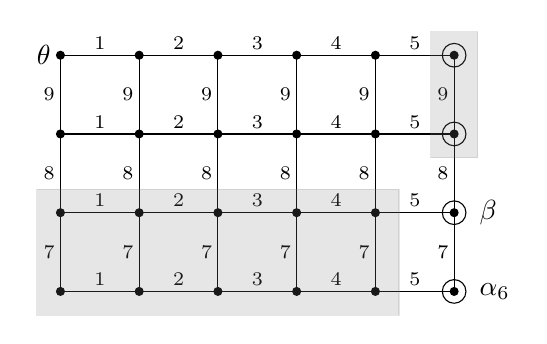
\begin{tikzpicture}[scale=1]
\foreach\x in{1,...,6} \draw(\x,6)--(\x,9); 
\foreach\y in{6,...,9} \draw(1,\y)--(6, \y);
\foreach\y in{6,...,9} \foreach\x in{1,...,6} 
\filldraw (\x,\y) circle(0.05cm);
\foreach\y in {6,...,9}
\draw (6,\y) circle(0.15cm);
\foreach\x in{1,...,6} \foreach\y in{7,...,9}
\node[left] at (\x+0.05, \y-.5) {$\ssty\y$};
\foreach\x in{1,...,5} \foreach\y in{6,...,9}
\node[above] at (\x+.5, \y-.05) {$\ssty\x$};
\node[right] at (6.2,7) {$\be$}; 
\filldraw[gray,opacity=0.2] (.7,7.3) rectangle (5.3, 5.7);
\filldraw[gray,opacity=0.2] (5.7,9.3) rectangle (6.3, 7.7);
\node[left] at (1,9) {$\theta$}; 
\node[right] at (6.2,6) {$\al_6$}; 
\end{tikzpicture}
$$
\caption{$I\cong \mathrm A_{9, 6}$, $\be=\al_{[6
, 7]}$. The gray boxes cover the roots in $H=(\check\omega_6-\check\omega_5-\check\omega_8)^\perp$.\label{fig:A}}
\end{figure}

\bigskip

\nl {\bf C.} $I\cong\mathrm C_{n, n}$. 
We recall that $\Phi^+=\{\al_{[i,j]},\ \al_{[i,n]}+\al_{[j,n-1]}\mid 1\leq i\leq j\leq n\}$,  hence $I=\{\al_{[i,n]}+\al_{[j,n-1]}\mid 1\leq i\leq j\leq n\}$ (with $\al_{[n,n-1]}=\nullvec$).

\par
We define $(S_I, \preq)=(\al_{[i,n]}| i=n,n-1, \dots, 1)$.
Then, $I\smeno S_I$ is the principal ideal $({\al_{n}+2\al_{n-1}}^\leq)$ of $\Phi^+$, in particular it is saturated.
Let $H_I=(2\check\omega_n-\check\omega_{n-1})^\perp$. 
It is easily seen that $\gen(I\smeno S_I)=H_I$ and 
$\al_{[1,n]} \not\in H_I$, hence $S_I$ is well defined.

\par
Now, we prove that $\be$ is detachable in  $(\be^\preq)$, for all $\be\in S_I$.

\par
Let $\be=\al_{[j,n]}$, with $j\in[1,n]$, $H=(2\check\omega_n-\check\omega_{n-1}-\check\omega_{j-1})^\perp$.
It is easy to check that  $\be$ is minimal in  $(\be^\preq)$.
We prove that $H$ is a detaching hyperplane.
Let $\Pi_1=\{\al_n+2\al_{n-1}\}\cup \{\al_i\mid j\leq i\leq n-2\}$, if $j\leq n-1$, and $\Pi_1=\emptyset$ \ if $j=n$.
Moreover, let $\Pi_2=\{\al_{[j-1,n]}\}\cup\{\al_i\mid 1\leq i\leq j-2\}$, if $j\leq 2$, and $\Pi_2=\emptyset$ for $i=1$.
Then, $\Pi_1\sqcup \Pi_2$ is a simple system for $\Phi\cap H$. 
Moreover, $\Phi\cap H=\Phi(\Pi_1)\cup \Phi(\Pi_2)$ is a decomposition into irreducible components (of type $\mathrm C$ and $\mathrm A$, respectively).  
It is easily seen that $I\cap \Phi(\Pi_1)$ and $I\cap \Phi(\Pi_2)$ are
element-wise incomparable, hence, the conditions of
Lemma~\ref{lem:simclosed-suff-cond} are satisfied, with $\Psi=\Phi\cap
H$. It follows that $I\cap H$ is $\sim$closed.

\par
If $\ga\in I$,  then $\ga=\al_{[h,n]}+\al_{[k, n-1]}$ for some $1\leq h\leq k\leq n$. 
Hence, $\ga\in H$ if and only if either $h\leq j-1$ and $k=n$, or $j\leq h\leq k\leq n-1$. 
In these cases, either $\ga$ and $\be$ are incomparable for the standard partial order,  or $\ga-\be\in \Phi^+$.
Moreover, if $\ga-\be\in \Phi^+$, then all $\ga'$ such that  $\ga<\ga'<\be$ are short roots. 
Hence, in any case, $\ga\nosim\be$,  by Proposition~\ref{pro:minori-crossing}\ref{itm:sim-then-nonroot}. 
If $\ga\in (\be^\preq)\smeno H$, we have  $\ga=\al_{[h,n]}+\al_{[k, n-1]}$ with $h\leq j-1\leq k\leq n-1$.
Then, $\be+\al_{[k,n-1]}\in\Phi$ and we obtain the  crossing relation $\be+\ga=(\be+\al_{[k,n-1]})+\al_{[h,n]}$.
It follows that $H$ satisfies the conditions of
Definition~\ref{def:detachable}, hence $\be$ is detachable in
$(\be^\preq)$   (see Figure~\ref{fig:C}).

\begin{figure}[hpt]
$$
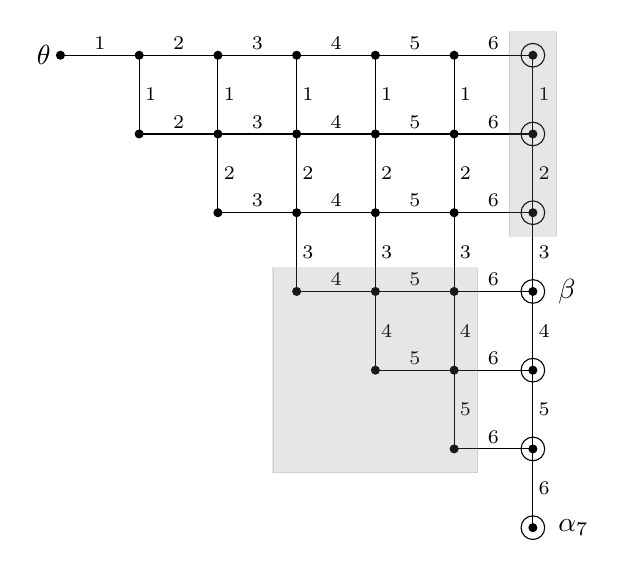
\begin{tikzpicture}[scale=1]
\foreach\x in{1,...,7} \draw(\x,-1)--(\x,-\x); 
\foreach\y in{-1,...,-7} \draw(7, \y)--(-\y,\y);
\foreach\x in {1,...,7}
\foreach\y in {-\x, ..., -1}
\filldraw (\x,\y) circle(0.05cm);
\foreach\x in {1,...,6}
\foreach\y in {-1, ..., -\x}
\node[above] at (\x+.5,\y-.05) {$\ssty\x$};
\foreach\y in {1,...,6}
\foreach\x in {\y,...,6}
\node[right] at (\x+0.95,-\y-.5) {$\ssty\y$};
\foreach\y in {-1,..., -7}
\draw (7,\y) circle(0.15cm);
\filldraw[gray,opacity=0.2] (3.7,-3.7) rectangle (6.3, -6.3);
\filldraw[gray,opacity=0.2] (6.7,-.7) rectangle (7.3, -3.3);
\node[left] at (1,-1) {$\theta$}; 
\node[right] at (7.2,-7) {$\al_7$}; 
\node[right] at (7.2,-4) {$\be$}; 
\end{tikzpicture}
$$
\caption{$I\cong \mathrm C_{7, 7}$, $\be=\al_{[4, 7]}$. 
The gray boxes cover the roots in $H=(2\check\omega_7-\check\omega_3-\check\omega_6)^\perp$.
\label{fig:C}
}
\end{figure}

\bigskip

\nl {\bf B1} and  {\bf D1.} $I\cong \mathrm B_{n, 1}$, or $I\cong \mathrm D_{n, 1}$. 
In case $ \mathrm B_{n, 1}$, we have 
$$I=\{\al_{[1, i]}\mid  1\leq i\leq n\}\cup \{\al_{[1, n]}+\al_{[j,n]}\mid 2\leq j\leq n\}.$$
In case $ \mathrm D_{n, 1}$, we have 
$$I=\{\al_{[1, i]}\mid 1\leq i\leq n\}\cup\{\wh\al_{[1, n]}\}\cup \{\al_{[1, n]}+\al_{[j,n]}\mid 2\leq j\leq n-2\},$$ where $\wh\al_{[1, n]}=\al_{[1, n]}-\al_{n-1}$.

\par
We define $(S_I, \preq)=(\al_1, \theta)$.
Let $H_I=(\check\omega_2-\check\omega_1)^\perp$. 
Then $\gen(I\smeno S_I)=H_I$ and $\theta\not\in H_I$, hence $S_I$ is well defined.
Since $S_I$ consists of the minimum and the maximum of $I$, we have that $I\smeno S_I$ is saturated.
\par
Finally, for each $\be\in S_I$, $\be$ is either the minimum, or the maximum of $(\be^\preq)$, with respect to the standard partial order, hence $\be$ is detachable in  $(\be^\preq)$ by Lemma~\ref{lem:detachable}.

\begin{figure}[hpt]%Figure 2
$$
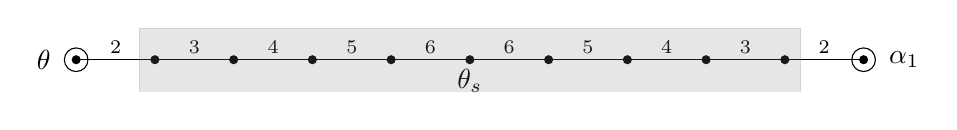
\begin{tikzpicture}[scale=1]
\draw(-5,0)--(5,0); 
\foreach\x in{-5,...,5} \filldraw (\x,0) circle(0.05cm);
\foreach\x in{2,...,6} 
\node[above] at (\x-6.5, -0.05) {$\ssty \x$};
\foreach\x in{2,...,6} 
\node[above] at (-\x+6.5, -0.05) {$\ssty \x$};
\node[right] at (5.2,0){$\al_1$};
\node[below] at (0,0){$\theta_s$};
\node[left] at (-5.2,0){$\theta$};
\foreach\x in{-5, 5}\draw (\x,0) circle(0.15cm);
\filldraw[gray, opacity=0.2] (-4.2, -.4) rectangle (4.2, .4);
\end{tikzpicture}
$$

$$%Figure 3
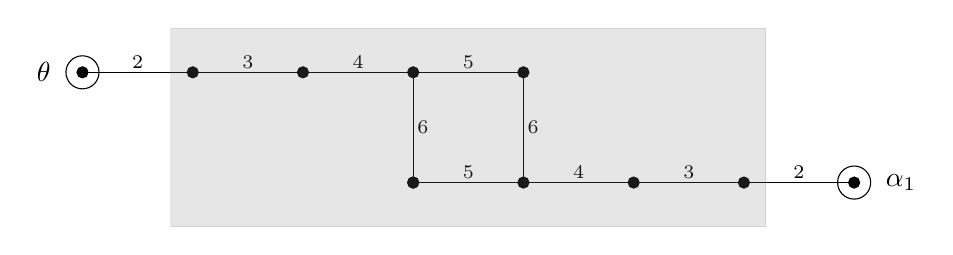
\begin{tikzpicture}[scale=1.4]
\draw(-4,0)--(0,0); 
\draw(-1,-1)--(3,-1); 
\draw(-1,0)--(-1,-1); 
\draw(0,0)--(0,-1); 
\foreach\x in{-4,...,0} \filldraw (\x,0) circle(0.05cm);
\foreach\x in{-1,...,3} \filldraw (\x,-1) circle(0.05cm);
 \filldraw (-1,-1) circle(0.05cm);
\foreach\x in {2,...,5}\node[above] at (\x-5.5, -0.05) {$\ssty \x$};
\foreach\x in {2,...,5}\node[above] at (-\x+4.5, -1.05) {$\ssty \x$};
\foreach\x in{-1,...,0} \node[right] at (\x-0.05, -0.5) {$\ssty 6$};
\node[right] at (3.2,-1){$\al_1$};
\node[left] at (-4.2,0){$\theta$};
\draw (-4,0) circle(0.15cm);
\draw (3,-1) circle(0.15cm);
\filldraw[gray, opacity=0.2] (-3.2, .4) rectangle (2.2, -1.4);
\end{tikzpicture}
$$
\caption{$I\cong \mathrm B_{6, 1}$ and $I\cong \mathrm D_{6, 1}$. In both cases, $S_I=\{\al_1, \theta\}$. 
The gray boxes cover the roots in $I\smeno S_I=I\cap H$, with $H=(\check\omega_1-\check\omega_2)^\perp$. 
\label{fig:BD1}}
\end{figure}

\bigskip

\nl {\bf Dn.} $I\cong\mathrm D_{n, n}$. 
Let $\wh\al_{[j,n]}=\al_{[j, n]}-\al_{n-1}$, for $1\leq j\leq n-1$.
Then, 
\begin{multline*}
I=
\{\wh\al_{[j,n]}\mid 1\leq j\leq n-1\} \cup \{\al_{[j,n]}\mid 1\leq j\leq n-2\}\, \cup \\
\{\al_{[i,n]}+\al_{[j,n-2]}\mid 1\leq i< j\leq n-2\}.
\end{multline*}
We define $(S_I, \preq)=(\wh\al_{[j,n]}| j=n,n-2, \dots, 1)$ and take $H_I=(\check\omega_n\smeno\check\omega_{n-1})^\perp$.
Then, $I\smeno S_I$ is the principal ideal $({\al_{[n-2,n]}}^\leq)$ of $\Phi^+$, hence it is saturated.
Moreover, we have $\gen(I\smeno S_I)=H_I$ and $\wh\al_{[1,n]}\not\in H_I$, hence $S_I$ is well defined.

\par
It remains to prove that, for all $\be\in S_I$, either one or the other of conditions (a) and (b) of Definition~\ref{def:triang-order}~\ref{itm:esterno} is satisfied.
If $\be=\al_n$ or $\be=\al_{n}+\al_{n-2}$, then $\be$ is the minimum of $(\be^\preq)$, hence it is detachable in  $(\be^\preq)$ by  Lemma~\ref{lem:detachable}. 
Then, let $\be=\wh\al_{[j,n]}$, with $j\in\{1,\dots,n-3\}$.
Let $J_{\mathrm f}=(\be^\leq)$. 
For $j>1$, let $\theta_{j-i}=\al_{[j-1,n]}+\al_{[j,n-2]}$, and $J_{\mathrm i}=(\be^\preq)\smeno (\theta_{j-1}^\leq) $ (see Figure~\ref{fig:D88-1}). 
For $j=1$, let  $J_{\mathrm i}=(\be^\preq)$: in this case $J_{\mathrm f}\subseteq J_{\mathrm i}$.
We prove that, for $j>1$,  $(\be^\preq)=J_{\mathrm i}\cup J_{\mathrm f}$ is a proper bipartition.
Indeed, we have: $(\be^\preq)=\{\ga\in I\mid c_{\al_j}(\ga)\geq 1 \text { or }  c_{\al_{n-1}}(\ga)\geq 1\}$, $J_{\mathrm i}\smeno J_{\mathrm f}=\{\ga\in I\mid c_{\al_j}(\ga)=0 \text{ and } c_{\al_{n-1}}(\ga)=1\}$, and $J_{\mathrm f}\smeno J_{\mathrm i}=\{\ga\in I\mid c_{\al_j}(\ga)=2\}$ (note that $c_{\al_j}(\ga)=2$ forces $c_{\al_n-1}(\ga)=1$). 
Hence, if we set $H=(\check\omega_n-\check\omega_j)^\perp$, $H$ strictly separates $J_{\mathrm i}\smeno J_{\mathrm f}$ from $J_{\mathrm f}\smeno J_{\mathrm i}$, and $J_{\mathrm i}\cap J_{\mathrm f}=I\cap H$. 
Moreover, for any $\ga_1\in J_{\mathrm i}\smeno J_{\mathrm f}$ and $\ga_2\in J_{\mathrm f}\smeno J_{\mathrm i}$ we have $c_{\al_j}(\ga_2-\ga_1)=2$ and $c_{\al_{n-1}}(\ga_2-\ga_1)=0$. 
This implies $\ga_2-\ga_1\not\in \Phi$, hence  $\ga_1\lesssim \ga_2$ by Proposition~\ref{pro:minori-crossing}\ref{itm:nonroot-then-sim}.
\par 
By  definition, we have $\be=\min J_\mathrm f$ hence we may apply Lemma~\ref{lem:detachable} with $J=J_{\mathrm f}$ and obtain that $\be$ is detachable in $J_\mathrm f$.
\enlargethispage{10cm}%
\par
The proof that $\be$ is also detachable in  $J_{\mathrm i}$ is very similar to the proofs of cases~$\mathrm A_{n}$ and $\mathrm C_n$.
We take  $H^{\mathrm i} =(\check\omega_n-\check\omega_{n-1}-\check\omega_{j-1})^\perp$, with $\check\omega_{0}=0$. 
Then, for each $\ga\in(\be^\preq)$, if $\ga\notin H^{\mathrm i}$ and $\ga\neq \be$, we have $\ga> \be$ and $(\ga, \be)=0$. 
If $\ga\in H^{\mathrm i}$, then either $\ga$ is incomparable with $\be$, or $\ga-\be\in \Phi$. 
Hence, by Corollary~\ref{cor:minori-crossing}, $\ga\sim\be$ if and only if $\ga\not\in H^{\mathrm i}$. 
It remains to prove that $I\cap H^{\mathrm i}$ is $\sim$closed.
Indeed, let  $\Pi_1=\{\al_{[n-1,n]}\}\cup\{\al_i\mid j\leq i\leq n-2\}$ and $\Pi_2=\{\wh\al_{[j-1,n]}\}\cup \{\al_i\mid 1\leq i\leq j-2\}$ ($\Pi_2=\emptyset$ for $j=1$).
Then, $\Pi_1\cup \Pi_2$ is a  simple system for $\Phi\cap H^{\mathrm i}$, and $\Phi\cap H^{\mathrm i}=\Phi(\Pi_1)\cup \Phi(\Pi_2)$ is a decomposition into irreducible components (of types $\mathrm D$ and $\mathrm A$, respectively, for $j>1$. For $j=1$ we have only the component $\Phi(\Pi_1)$, which is irreducible of type $\mathrm D_{n-1}$).  
It is easy to see that $I\cap \Phi(\Pi_1)$ and $I\cap \Phi(\Pi_2)$ are
pairwise incomparable, hence we may apply
Lemma~\ref{lem:simclosed-suff-cond} with $\Psi=\Phi\cap H^{\mathrm i}$
and obtain that $I\cap \Psi= I\cap H^{\mathrm i}$ is~$\sim$closed.
%(see Figures~\ref{fig:D88-1}, \ref{fig:D88-2}).
\begin{figure}[hbtp]%Figure 4
$$
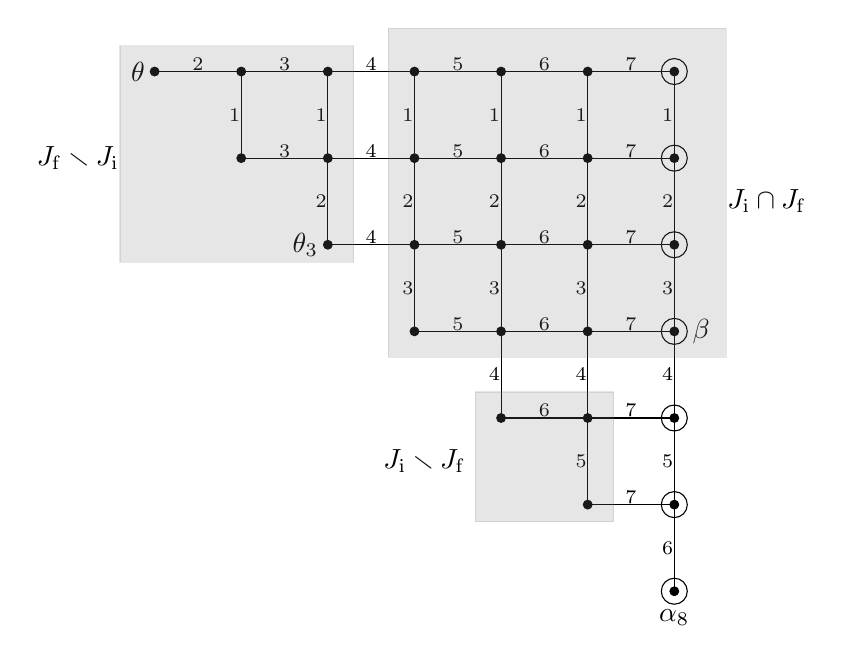
\begin{tikzpicture}[scale=1.1]
\foreach\x in{0,...,6}  \draw(\x, -\x)--(6, -\x); 
\foreach\x in{0,...,6}  \draw(\x, -\x)--(\x, 0); 
\foreach\x in{0,...,6} \foreach\y in{-\x, ..., 0} 
\filldraw (\x,\y) circle(0.05cm);
\foreach\y in {1, ...,6} \foreach\x in{\y,...,6} 
\node[left]at (\x+.1, -\y+0.5) {$\ssty \y$};
\foreach\x in {2, ...,7} \foreach\y in{-\x,...,-2} 
\node[above] at (\x- 1.5, \y+1.9) {$\ssty \x$};
\node[below] at (6,-6.1){$\al_8$};
\node[left] at (0,0){$\theta$};
\node[left] at (2,-2){$\theta_3$};
\node[right] at (6.1,-3) {$\be$}; 
\foreach\y in{-6, ..., 0}\draw (6,\y) circle(0.15cm);
\filldraw[gray, opacity=0.2] (-.4,.3) rectangle (2.3, -2.2);
\node[left] at (-0.3,-1) {$J_{\mathrm f}\smeno J_{\mathrm i}$}; 
\filldraw[gray, opacity=0.2] (3.7,-3.7) rectangle (5.3, -5.2);
\node[left] at (3.7,-4.5) {$J_{\mathrm i}\smeno J_{\mathrm f}$}; 
\filldraw[gray,opacity=0.2] (2.7,.5) rectangle (6.6, -3.3);
\node[right] at (6.5,-1.5) {$J_{\mathrm i}\cap J_{\mathrm f}$}; 
\end{tikzpicture}
$$
\caption{$I\cong \mathrm D_{8,8}$, $\be=\wh\al_{4, 8}$.  
The gray boxes cover $(\be^\preq)$, partitioned according to the bipartition described in the proof. 
\label{fig:D88-1}}
\end{figure}
\clearpage
\begin{figure}[tbp]%Figure5
$$
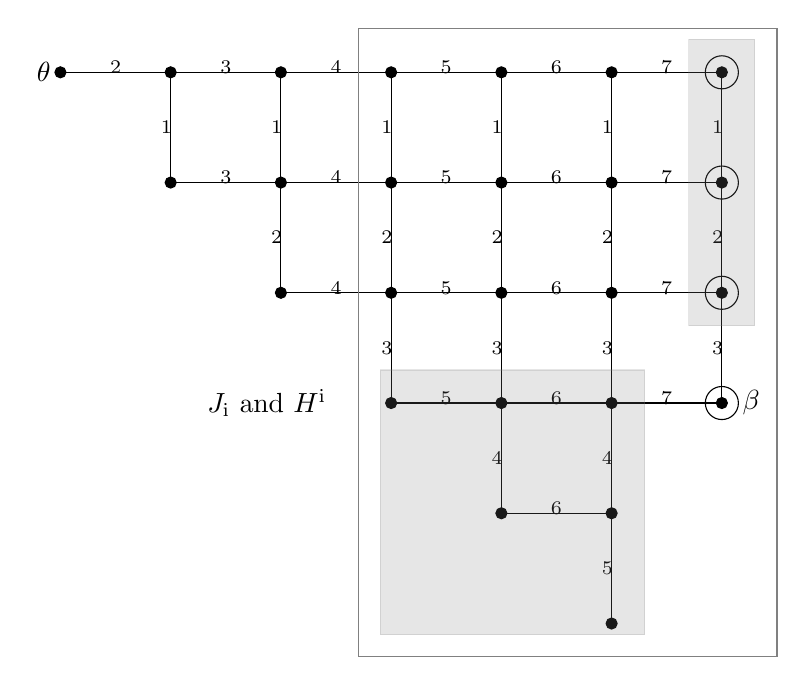
\begin{tikzpicture}[scale=1.4]
\foreach\x in{0,...,3}  \draw(\x, -\x)--(6, -\x); 
\foreach\x in{4,...,5}  \draw(\x, -\x)--(5, -\x); 
\foreach\x in{0,...,5}  \draw(\x, -\x)--(\x, 0); 
\draw(6, -3)--(6, 0); 
\foreach\x in{0,...,5} \foreach\y in{-\x, ..., 0} 
\filldraw (\x,\y) circle(0.05cm);
\foreach\y in{-3, ..., 0}
\filldraw (6,\y) circle(0.05cm);
\foreach\y in {1, ...,5} \foreach\x in{\y,...,5} 
\node[left]at (\x+.1, -\y+0.5) {$\ssty \y$};
\foreach\y in {1, ...,3} 
\node[left]at (6.1, -\y+0.5) {$\ssty \y$};
\foreach\x in {2, ...,6} \foreach\y in{-\x,...,-2} 
\node[above] at (\x- 1.5, \y+1.9) {$\ssty \x$};
\foreach\y in{-3,...,0} 
\node[above] at (5.5, \y-.1) {$\ssty 7$};
\node[left] at (0,0){$\theta$};
\node[right] at (6.1,-3) {$\be$}; 
\foreach\y in{-3, ..., 0}\draw (6,\y) circle(0.15cm);
\draw[gray] (2.7,.4) rectangle (6.5, -5.3);
\filldraw[gray, opacity=0.2] (2.9,-2.7) rectangle (5.3, -5.1);
\filldraw[gray, opacity=0.2] (5.7,.3) rectangle (6.3, -2.3);
\node[left] at (2.5,-3) {$J_{\mathrm i}$ and $H^{\mathrm i}$}; 
\end{tikzpicture}
$$
\caption{$I\cong \mathrm D_{8,8}$, $\be=\widehat\al_{4, 8}$.  
The diagram represents $(\be^\preq)$. 
The big rectangle contains the roots in $J_{\mathrm i}$
and the gray parts cover the roots in $H^{\mathrm i}=(\check\omega_8-\check\omega_7-\check\omega_3)^\perp$.
\label{fig:D88-2}}
\end{figure}

\bigskip
\nl {\bf E6.} $I\cong \mathrm E_{6, 6}$. 
We choose  
$$(S_I,\preq)=\left(\al_6, \theta, \al_{\{5,6\}}, \theta-\al_2, \al_{\{4,5,6\}}, \theta-\al_{\{2,4\}}, \al_{\{2,4,5,6\}}, \theta-\al_{\{2, 4, 5\}}\right).$$
The roots in $(S_I,\preq)$ are all the $\ga\in I$ with $c_{\al_3}(\ga)=0$, alternated with their symmetric roots with respect to the order involution, which are all the $\ga\in I$ with $c_{\al_3}(\ga)=2$.
Hence $I\smeno S_I$ is saturated.

\par
Let $H_I=(\check\omega_6-\check\omega_3)^\perp$. 
Then, $\gen(I\smeno S_I)= H_I$ and  $\theta-\al_{\{2, 4, 5\}}\not\in H_I$, hence $S_I$ is well defined.

\par
Let $\Pi'=\{\al_{[3,6]}\}\cup \Pi\smeno\{\al_3, \al_6\}$.
Then $\Phi(\Pi')$ is irreducible, of type $\mathrm A_5$, and  $I\smeno S_I$ is the abelian nilradical generated by $\al_{[3,6]}$
in $\Phi(\Pi')$, of type $\mathrm A_{5,2}$. 
Hence, $I\cap\gen(I\smeno S_I)$ is $\sim$closed by Lemma~\ref{lem:simclosed-suff-cond} applied with $\Psi=\Phi(\Pi')$. 

\par
The first six $\be$ in $(S_I,\preq)$ are detachable in  their $(\be^\preq)$ by Lemma~\ref{lem:detachable}, being either the minimum, or the maximum of $(\be^\preq)$. 
Hence, it remains to prove that the last two roots, $\be=\al_{\{2,4,5,6\}}$ and $\be'=\theta-\al_{\{2, 4, 5\}}$ are detachable in their $\preq$-cone.
We will prove that, in both cases, $H_I$ is a detaching hyperplane.
We have $(\be^\preq)=\{\be\}\cup (I\smeno S_I)\cup \{\be'\}$.
It is easy to check that, for all $\ga\in I\smeno S_I$, either $\be$ is incomparable with $\ga$, or $\ga-\be\in \Phi^+$.
Hence, by Corollary~\ref{cor:minori-crossing},  $\be\not\sim\ga$ for all $\ga\in I\smeno S_I$.  
For $\be'$, we have $\be\leq \be'$ and $\be'-\be\not\in \Phi$, hence $\be\lesssim \be'$.
Now, $H_I$ strictly separates $\be$ from $\be'$ since $c_{\al_3}(\be)=0$ and $c_{\al_3}(\be')=2$. 
Morever, we have already seen that $I\smeno S_I$ is equal to $I\cap H_I$ and is  saturated, hence $\sim$closed. 
It follows that $\be$ is detached in $(\be^\preq)$, with detaching hyperplane $H_I$.
For $\be'$, the proof is similar  (see Figure~\ref{fig:E66}).
\begin{figure}[tp]
$$
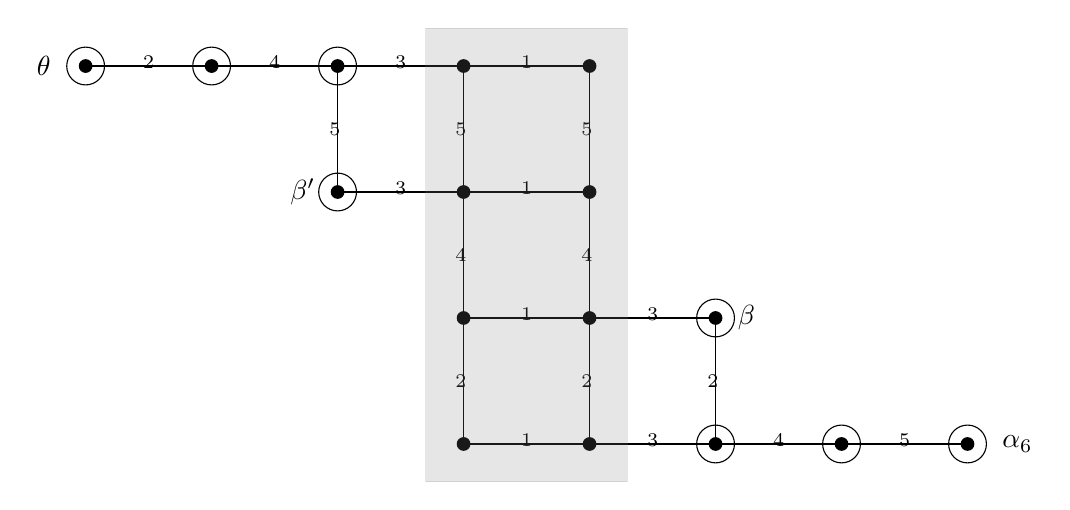
\begin{tikzpicture}[scale=1.6]%Figure 6
\draw (0,0)--(0,3);
\draw (0,1)--(2,1);
\draw (-1,2)--(1,2);
\draw (-3,3)--(1,3);
\draw (-1,2)--(-1,3);
\draw (0,0)--(4,0);
\draw (1,0)--(1,3);
\draw (2,0)--(2,1);
\foreach\x in {0, ..., 4}
\filldraw(\x,0) circle(0.05cm);
\foreach\x in {0, ..., 2}
\filldraw(\x,1) circle(0.05cm);
\foreach\x in {-1, ..., 1}
\filldraw(\x,2) circle(0.05cm);
\foreach\x in {-3, ..., 1}
\filldraw(\x,3) circle(0.05cm);
\node[above] at (-2.5,2.9)  {$\ssty 2$};
\node[above] at (-1.5,2.9)  {$\ssty 4$};
\foreach\y in {2,...,3}\node[above] at (-0.5,\y-.1) {$\ssty 3$};
\foreach\y in {0,...,3}\node[above] at (0.5,\y-.1) {$\ssty 1$};
\foreach\y in {0,...,1}\node[above] at (1.5,\y-.1) {$\ssty 3$};
\node[above] at (2.5,-.1)  {$\ssty 4$};
\node[above] at (3.5,-.1)  {$\ssty 5$};
\foreach\x in {-1,...,1}\node[left] at (\x+.1,2.5) {$\ssty 5$};
\foreach\x in {0,...,1}\node[left] at (\x+.1,1.5) {$\ssty 4$};
\foreach\x in {0,...,2}\node[left] at (\x+.1,0.5) {$\ssty 2$};
\node[left] at (-3.2,3)  {$\theta$};
\node[right] at (4.2,0)  {$\al_6$};
\foreach \x in {2,3,4}\draw (\x,0) circle(0.15cm); 
\foreach \x in {-3,-2,-1}\draw (\x,3) circle(0.15cm); 
\draw (-1,2) circle(0.15cm); 
\draw (2,1) circle(0.15cm); 
\filldraw[gray, opacity=0.2](-.3,3.3) rectangle (1.3,-.3);
\node[right] at (2.1, 1) {$\be$};
\node[left] at (-1.1, 2) {$\be'$};
\end{tikzpicture}
$$
\caption{
$I\cong \mathrm E_{6,6}$, $\be=\al_{\{2,4,5,6\}}$, and $\be'=\theta-\al_{\{2,4,5\}}$. 
The gray rectangle covers the roots in  $H_I=(\check\omega_6-\check\omega_3)^\perp$. 
\label{fig:E66}}
\end{figure}

\bigskip

\nl {\bf E7.} $I\cong \mathrm E_{7, 7}$. 
We recall that $\theta=2\al_1+2\al_2+3\al_3+4\al_4+3\al_5+2\al_6+\al_7$. 
The order involution maps $\al_2$ and $\al_4$ onto their opposite roots, $\al_7$ onto $\theta$, and the sequence $(\al_1, \al_3,\al_5, \al_6)$ onto $(-\al_6, -\al_5, -\al_3, -\al_1)$.
\par
For any $\ga\in I$, we denote by $\ga'$ the symmetric of $\ga$ with respect to the order involution and we define
\begin{align*}
(S_I, \preq)=
(&\al_7,\: \al_7',\: 
\al_{\{6, 7\}},\ \al_{\{6, 7\}}',\ 
\al_{\{5, 6,7\}},\ \al_{\{5, 6,7\}}',\ 
\al_{\{4, 5, 6,7\}},\ \al_{\{4, 5, 6,7\}}',\ 
\al_{\{2, 4, 5, 6,7\}},\\
&\al_{\{2, 4, 5, 6,7\}}',\ 
\al_{\{3, 4, 5, 6,7\}},\ \al_{\{3, 4, 5, 6,7\}}',\ 
\al_{\{1, 3, 4, 5, 6,7\}},\ \al_{\{1, 3, 4, 5, 6,7\}}').
\end{align*}
By definition, $(S_I,\preq)$ consists of all $\be$ in $I$ such that $c_{\al_2}(\be)+c_{\al_3}(\be)\leq 1$, together with their symmetric roots  (see Figure~\ref{fig:E77-1}).
Then, we have $\min(I\smeno S_I)=\al_{[2,7]}$, hence $\max(I\smeno S_I)=\al_{[2,7]}'$. 
In particular,  $I\smeno S_I$ is a root interval, hence it is saturated.

\par
Let $H_I=(\check\omega_7-\check\omega_2)^\perp$ and let $\be=\al_{\{2, 4, 5, 6,7\}}$. 
We can directly check that $H_I\cap I=(I\smeno S_I)\cup \{\be, \be'\}$. 
We have $\be, \be'\in S_I$, nevertheless, $\gen(I\smeno S_I)=H_I$.
Moreover, $\max_\preq S_I=\al_{\{1, 3, 4, 5, 6,7\}}'=\theta-\al_{\{1, 3, 4, 5, 6\}}\not\in H_I$. 
Hence, $S_I$ is well defined (see Figure~\ref{fig:E77-1}).

\begin{figure}[htbp]
$$
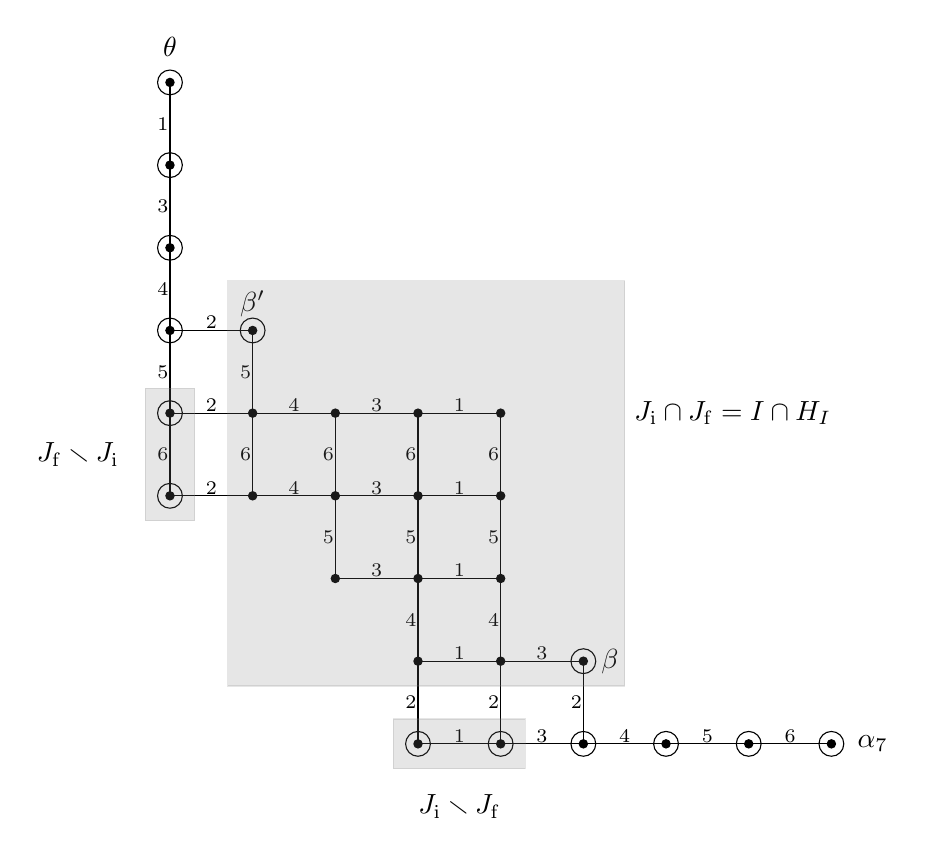
\begin{tikzpicture}[scale=1.05]
\draw (-4,4)--(-4,-1);
\draw (-1,-4)--(4,-4);
\draw (-4,1)--(-3, 1)--(-3, -1);
\foreach\y in{0, -1}\draw (-4,\y)--(0,\y);
\foreach\x in{0, -1}\draw (\x,0)--(\x,-4);
\draw(-2, 0)--(-2, -2)--(0, -2);
\draw (-1,-3)--(1,-3)--(1, -4);
\node[left] at (-3.9,3.5)  {$\ssty 1$};
\node[left] at (-3.9, 2.5)  {$\ssty 3$};
\node[left] at (-3.9, 1.5)  {$\ssty 4$};
\foreach\x in {-4,-3}\node[left] at (\x+.1,0.5)  {$\ssty 5$};
\foreach\x in {-4,...,0}\node[left] at (\x+.1,-0.5)  {$\ssty 6$};
\foreach\x in {-2,..., 0}\node[left] at (\x+.1,-1.5)  {$\ssty 5$};
\foreach\x in {-1,0}\node[left] at (\x+.1,-2.5)  {$\ssty 4$};
\foreach\x in {-1,..., 1}\node[left] at (\x+.1,-3.5)  {$\ssty 2$};
\node[above] at (3.5,-4.1)  {$\ssty 6$};
\node[above] at (2.5,-4.1)  {$\ssty 5$};
\node[above] at (1.5,-4.1)  {$\ssty 4$};
\foreach\y in {-4,-3}\node[above] at (0.5,\y-.1)  {$\ssty 3$};
\foreach\y in {-4,...,0}\node[above] at (-0.5,\y-.1)  {$\ssty 1$};
\foreach\y in {-2,..., 0}\node[above] at (-1.5,\y-.1)  {$\ssty 3$};
\foreach\y in {-1,0}\node[above] at (-2.5,\y-.1)  {$\ssty 4$};
\foreach\y in {-1,..., 1}\node[above] at (-3.5,\y-.1)  {$\ssty 2$};
\foreach\y in {-1,...,4}
\filldraw(-4,\y) circle(0.05cm);
\foreach\x in {-1,...,4}
\filldraw(\x,-4) circle(0.05cm);
\foreach\x in {-1,...,1}
\filldraw(\x, -3) circle(0.05cm);
\foreach\y in {-1,...,1}
\filldraw(-3, \y) circle(0.05cm);
\foreach\x in {-2,...,0}\foreach\y in {-2,...,0}
\filldraw(\x, \y) circle(0.05cm);
\node[above] at (-4,4.2) {$\theta$}; 
\node[right] at (4.2,-4) {$\al_7$}; 
\foreach\y in {-1, ..., 4} 
\draw(-4, \y) circle (0.15cm); 
\foreach\x in {-1, ..., 4} 
\draw(\x, -4) circle (0.15cm); 
\draw(1, -3) circle (0.15cm); 
\draw(-3,1) circle (0.15cm); 
\node[right] at (1.1,-3){$\be$};
\node[above] at (-3,1.05){$\be'$};
\filldraw[gray, opacity=0.2] (-3.3, 1.6)rectangle(1.5, -3.3); 
\node[right]at(1.5,0){$J_{\mathrm i}\cap J_{\mathrm f}=I\cap H_I$};
\filldraw[gray, opacity=0.2] (-4.3, .3)rectangle(-3.7, -1.3); 
\node[left]at(-4.5,-.5){$J_{\mathrm f}\smeno J_{\mathrm i}$};
\filldraw[gray, opacity=0.2] (.3,-4.3)rectangle(-1.3,-3.7); 
\node[below]at(-.5,-4.5){$J_{\mathrm i}\smeno J_{\mathrm f}$};
\end{tikzpicture}
$$
\caption{$I\cong \mathrm E_{7, 7}$, $\be=\al_{\{2,4,5,6,7,\}}$. The gray rectangles illustrate the bipartition of $(\be^\preq)$. 
For the symmetric root $\be'=\theta-\al_{[1,4]}$, the bipartition of $(\be'^\preq)$ is similar. 
\label{fig:E77-1}}
\end{figure}

\par
All roots in $S_I$, except $\be=\al_{\{2, 4, 5, 6,7\}}$, $\eta=\al_{\{1, 3, 4, 5, 6,7\}}$ and their symmetric roots, are either the minimum, or the maximum of their $\preq$-upper cone, with respect to the standard partial order, so they are detachable in it by Lemma~\ref{lem:detachable}. 
It remains to consider $\be, \be', \eta, \eta'$.

\par
First, we find a bipartition of  $(\be^\preq)$ that satisfies the requirements of Definition~\ref{def:triang-order}\ref{itm:esterno}. 
Let $J_{\mathrm f}=(\be^\preq)\cap (\be^\leq) =\{\ga\in (\be^\preq)\mid c_{\al_2}(\ga)\geq 1\}$ and $J_{\mathrm i}=\{\ga\in (\be^\preq)\mid c_{\al_2}(\ga)\leq 1\}$. 
It is easily seen that $J_{\mathrm i}\cap J_{\mathrm f}=I\cap H_I$ and that $H_I$ strictly separates $J_{\mathrm i}\smeno J_{\mathrm f}$ from $J_{\mathrm f}\smeno J_{\mathrm i}$. 
Moreover, we can directly check that,  for all $\ga_1\in J_{\mathrm i}\smeno J_{\mathrm f}$ and $\ga_2\in J_{\mathrm f}\smeno J_{\mathrm i}$, we have $\ga_2-\ga_1 \in 
L^+(\Phi)\smeno \Phi^+$, hence $\ga_1\lesssim \ga_2$. 
It remains to check that $\be$ is detachable in  $J_{\mathrm i}$ and $J_{\mathrm f}$.
For $J_{\mathrm f}$ this follows from Lemma~\ref{lem:detachable}, since $\be=\min_\leq J_{\mathrm f}$. 
For $J_{\mathrm i}$, we prove that the hyperplane  $H^{\mathrm i}=(\check\omega_7-\check\omega_3)^\perp$ is a detaching hyperplane. 
Indeed, $(\Phi\cap H^{\mathrm i})$ is an irreducible root subsystem of type $A_6$, with simple system $\{\al_{[3,7]}\}\cup \Pi\smeno\{\al_7, \al_3\}$. 
Hence, we may apply  Lemma~\ref{lem:simclosed-suff-cond}, with $\Psi=\Phi\cap H^{\mathrm i}$, and find that $I\cap H^{\mathrm i}$ is $\sim$closed (see also Figure \ref{fig:E77-2}). 
Moreover, we can directly check that, for all $\ga\in J_{\mathrm i} \cap H^{\mathrm i}$, either $\ga$ and $\be$ are incomparable, or $\ga - \be\in \Phi^+$, hence $\ga\not\sim \be$. 
Finally, for all $\ga\in J_{\mathrm i} \smeno H^{\mathrm i}$, we have $\ga> \be$ and $\ga-\be\not\in \Phi$, hence, by Corollary~\ref{cor:minori-crossing}, $\ga\sim \be$.
Hence $H^{\mathrm i}$ is a detaching hyperplane for $\be$ in
$J_{\mathrm i}$ (see Figure~\ref{fig:E77-2}).


\begin{figure}[btp]
\centering
$$
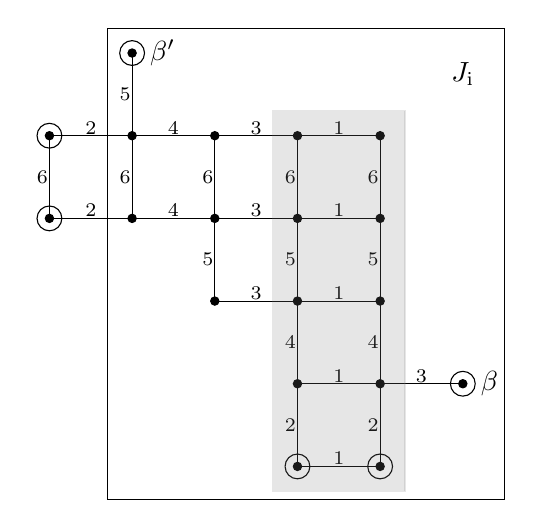
\begin{tikzpicture}[scale=1.05]
\draw (-4,0)--(-4,-1);
\draw (-1,-4)--(0,-4);
\draw (-3, 1)--(-3, -1);
\foreach\y in{0, -1}\draw (-4,\y)--(0,\y);
\foreach\x in{0, -1}\draw (\x,0)--(\x,-4);
\draw(-2, 0)--(-2, -2)--(0, -2);
\draw (-1,-3)--(1,-3);
\foreach\x in {-3}\node[left] at (\x+.1,0.5)  {$\ssty 5$};
\foreach\x in {-4,...,0}\node[left] at (\x+.1,-0.5)  {$\ssty 6$};
\foreach\x in {-2,..., 0}\node[left] at (\x+.1,-1.5)  {$\ssty 5$};
\foreach\x in {-1,0}\node[left] at (\x+.1,-2.5)  {$\ssty 4$};
\foreach\x in {-1,...,0}\node[left] at (\x+.1,-3.5)  {$\ssty 2$};
\foreach\y in {-3}\node[above] at (0.5,\y-.1)  {$\ssty 3$};
\foreach\y in {-4,...,0}\node[above] at (-0.5,\y-.1)  {$\ssty 1$};
\foreach\y in {-2,..., 0}\node[above] at (-1.5,\y-.1)  {$\ssty 3$};
\foreach\y in {-1,0}\node[above] at (-2.5,\y-.1)  {$\ssty 4$};
\foreach\y in {-1,..., 0}\node[above] at (-3.5,\y-.1)  {$\ssty 2$};
\foreach\y in {-1,...,0}
\filldraw(-4,\y) circle(0.05cm);
\foreach\x in {-1,...,0}
\filldraw(\x,-4) circle(0.05cm);
\foreach\x in {-1,...,1}
\filldraw(\x, -3) circle(0.05cm);
\foreach\y in {-1,...,1}
\filldraw(-3, \y) circle(0.05cm);
\foreach\x in {-2,...,0}\foreach\y in {-2,...,0}
\filldraw(\x, \y) circle(0.05cm);
\foreach\y in {-1, ..., 0} 
\draw(-4, \y) circle (0.15cm); 
\foreach\x in {-1, ..., 0} 
\draw(\x, -4) circle (0.15cm); 
\draw(1, -3) circle (0.15cm); 
\draw(-3,1) circle (0.15cm); 
\node[right] at (1.1,-3){$\be$};
\node[right] at (-2.9,1){$\be'$};
\draw (-3.3, 1.3)rectangle(1.5, -4.4); 
\node[below] at(1,1){$J_{\mathrm i}$};
\filldraw[gray, opacity=0.2] (-1.3,.3)rectangle(0.3,-4.3); 
\end{tikzpicture}
$$
\caption
{$I\cong \mathrm E_{7, 7}$, $\be=\al_{\{2,4,5,6,7,\}}$. The diagram represents  $(\be^\preq)$.  
The big rectangle contains the roots in $J_{\mathrm i}$ and the gray part covers the roots in $H^{\mathrm i}=(\check\omega_7-\check\omega_3)^\perp$. 
\label{fig:E77-2}}
\end{figure}


The case of  $\be'$ is similar to the previous one, by symmetry.


It remains to deal with $\eta$ and $\eta'$. 
In this case, $H_I$ is a detaching hyperplane for  $\eta$ in $(\eta^\preq)$ as well as for $\eta'$ in $({\eta'}^\preq)$
(see Figure \ref{fig:E77-3}).
Indeed, it is easily checked that for all $\ga\in (\eta^\preq)\cap H_I$, either $\ga$ is incomparable with $\eta$ and $\eta'$, or $\ga-\eta$, $\ga-\eta'\in \Phi$. 
Hence $\ga\not\sim\eta, \eta'$. 
Moreover, $(\eta^\preq)\smeno H_I=\{\eta, \eta'\}$, $H_I$ separates $\eta$ from $\eta'$, and $\eta\sim \eta'$.  
Finally, $(\eta'^\preq)\smeno H_I=\{\eta'\}$. 
This concludes the proof.
\end{proof}
\begin{figure}[hpt]
$$
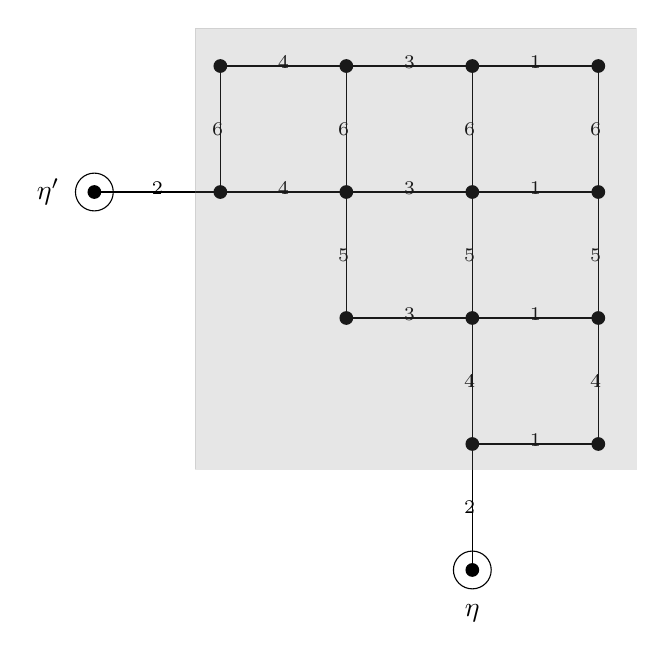
\begin{tikzpicture}[scale=1.6]
\draw (-3, 0)--(-3, -1);
\draw (-3,0)--(0,0);
\draw (-4,-1)--(0,-1);
\draw (0,-3)--(0,0);
\draw (-1,-4)--(-1,0);
\draw(-2, 0)--(-2, -2)--(0, -2);
\draw (-1,-3)--(0,-3);
\foreach\x in {-3,...,0}\node[left] at (\x+.1,-0.5)  {$\ssty 6$};
\foreach\x in {-2,..., 0}\node[left] at (\x+.1,-1.5)  {$\ssty 5$};
\foreach\x in {-1,0}\node[left] at (\x+.1,-2.5)  {$\ssty 4$};
\foreach\x in {-1}\node[left] at (\x+.1,-3.5)  {$\ssty 2$};
\foreach\y in {-3,...,0}\node[above] at (-0.5,\y-.1)  {$\ssty 1$};
\foreach\y in {-2,..., 0}\node[above] at (-1.5,\y-.1)  {$\ssty 3$};
\foreach\y in {-1,0}\node[above] at (-2.5,\y-.1)  {$\ssty 4$};
\foreach\y in {-1}\node[above] at (-3.5,\y-.1)  {$\ssty 2$};
\filldraw(-4,-1) circle(0.05cm);
\filldraw(-1,-4) circle(0.05cm);
\foreach\x in {-1,...,0}
\filldraw(\x, -3) circle(0.05cm);
\foreach\y in {-1,...,0}
\filldraw(-3, \y) circle(0.05cm);
\foreach\x in {-2,...,0}\foreach\y in {-2,...,0}
\filldraw(\x, \y) circle(0.05cm);
\draw(-4, -1) circle (0.15cm); 
\draw(-1, -4) circle (0.15cm); 
\node[below] at (-1,-4.2){$\eta$};
\node[left] at (-4.2,-1){$\eta'$};
\filldraw[gray, opacity=0.2] (-3.2,.3)rectangle(0.3,-3.2); 
\end{tikzpicture}
$$
\caption
{$I\cong \mathrm E_{7, 7}$, $\ga=\al_{\{1,3,4,5,6,7,\}}$. The diagram represents $(\eta^\preq)$. 
The gray square covers the roots contained in $H_I=(\check\omega_7-\check\omega_2)^\perp$. 
\label{fig:E77-3}}
\bigskip
\end{figure}

\section{Triangulations of standard parabolic facets}
\label{sec:triangulation}
In this section we prove Theorems~\ref{thm:main1-intro} and~\ref{thm:main2-intro}.

\par
Let $I$ be a face ideal of $\Phi^+$ and $F_I=\conv(I)$ be the corresponding standard parabolic face. 
For all $J\subseteq I$, let
$$
\mc R_J=\{R\subseteq J\mid R \text{ reduced}\}.
$$
Then, let
$$
\mc T_I=\{\conv(R)\mid R\in \mc R_I, R \text{ maximal in } \mc R_I\}.
$$
We will prove that $\mc T_I$ is a triangulation of  $\mathrm F_I$. 
\par
By Propositions~\ref{pro:abnil-are-facets} and~\ref{pro:faces-are-abnil}, it suffices to prove the 
claim when $I$ is an abelian nilradical of $\Phi^+$.  
Henceforward, we make this assumption. 
So, there exists a unique simple root $\al_I\in \Pi$ such that $m_{\al_I}=1$ and $I=(\al_I^\leq)$.
In particular, $I$ is a facet ideal and $F_I$ is a facet of $\pol$.
\par

The proof is by induction on $\rk(\Phi)$ and is based on the existence of triangulation orders for all facet ideals. 
We start with two key lemmas. 

\par
For each $J\subseteq I$ let $\cone(J)$ be the positive cone generated by $J$, i.e. the set of linear combinations of elements in $J$ with nonnegative real coefficients.
Moreover, let $[J]$ be the {\it saturation} of $J$, i.e. 
$$[J]=\{x\in I\mid \exists\, y,z\in J\ y\leq x\leq z\}.$$ 

%\smallskip

\begin{lem}\label{lem:coni-bipartite}
Let $J$ be a saturated subset of $I$, and  $\{J_{\mathrm i},J_{\mathrm f}\}$ be a  bipartition of $J$.
Then $\cone(J)=\cone(J_{\mathrm i})\cup \cone(J_{\mathrm f})$. 
\end{lem}

\begin{proof}
The claim is obvious if the bipartition is not proper, in particular if $|J|\leq 2$. 
The inclusion $\cone(J_{\mathrm i})\cup \cone(J_{\mathrm f})\subseteq \cone(J)$ is clear in all cases.
We prove the reverse inclusion by induction on $|J|$. 
It is easily seen that, for any $K\subseteq J$, $\{K\cap J_{\mathrm i}, K\cap J_{\mathrm f}\}$ is a bipartition of $K$.  
Therefore, it suffices to prove that if the bipartition $\{J_{\mathrm i},J_{\mathrm f}\}$ of $J$ is proper,  there exists a proper saturated subset $K$ of $J$ such that $x\in \cone(K)$. 
\par

So, let $J_{\mathrm i}, J_{\mathrm f}\subsetneqq J$, $x\in \cone(J)$, and $x=\sum\limits_{\be\in J}c_\be\be$,  with $c_\be$ nonnegative real coefficients, be a fixed expression of $x$.
If $\{\be\in J\mid c_\be> 0\}$ is included in $J_{\mathrm i}$ or $J_{\mathrm f}$ we are done.
Also if the saturation $[\{\be\in J\mid c_\be> 0\}]$ is properly included in $J$ we are done.
Hence, we assume  $J=[\{\be\in J\mid c_\be> 0\}]$. 
This means that, for all $\be\in \Min\, J\cup  \Max\, J$, $c_\be> 0$.
Since $J_{\mathrm i}\smeno J_{\mathrm f}$ and $J_{\mathrm f}\smeno J_{\mathrm i}$ are an initial and a final section of $J$, we have  $\Min(J_{\mathrm i}\smeno J_{\mathrm f})\subseteq \Min\, J$ and $\Max(J_{\mathrm f}\smeno J_{\mathrm i})\subseteq \Max\, J$.
We fix  $\be_1\in \Min (J_{\mathrm i}\smeno J_{\mathrm f})$ and $\be_2\in \Max(J_{\mathrm f}\smeno J_{\mathrm i})$.
By Definition~\ref{def:bipartite}, and since $J$ is saturated, there exist $\ga_1, \ga_2\in J$  such that $\be_1+\be_2=\ga_1+\ga_2$ and $\be_1< \{\ga_1, \ga_2\}< \be_2$. 
Hence, $c_{\be_1}\be_1+ c_{\be_2} \be_2=(c_{\be_1}-c_{\be_2}) \be_1 + c_{\be_2} (\ga_1+\ga_2) =$ $(c_{\be_2}-c_{\be_1}) \be_2 + c_{\be_1} (\ga_1+\ga_2)$.
We obtain that, if  $c_{\be_1}\geq  c_{\be_2}$, then $x\in \cone (J \smeno\{\be_2\})$, while, if  $c_{\be_2}\geq  c_{\be_1}$, then $x\in \cone (J \smeno\{\be_1\})$. 
Since $\be_1$ and $\be_2$ are extremal elements in $J$, $J \smeno\{\be_1\}$ and $J \smeno\{\be_2\}$ are saturated, hence the claim is proved.
\end{proof}

\begin{lem}\label{lem:coni-detachable}
Let $J$ be a saturated subset of $I$, $\be^*\in J$,  $\be^*$ detachable in  $J$, and $J_{\be^*}=\{\be^*\}\cup (\red(\be^*)\cap J)$. Then, $\cone(J)=\cone(J_{\be^*})\cup \cone(J\smeno\{\be^*\})$.
\end{lem}

\begin{proof}
Let $J'=J\smeno \red(\be^*)$. 
Then, $\cone(J)=\cone(J')+ \cone(\red(\be^*)\cap J)\subseteq
\cone(J')+ \cone(J_{\be^*}).$ 
Hence, it suffices to prove that $\cone(J')\subseteq \cone(J_{\be^*})\cup \cone(J\smeno\{\be^*\})$. 

\par
Let $x\in\cone(J')$,  $\mc K=\{K\subseteq J'\mid x\in \cone(K)\}$, and $d=\min\{|[K]|\mid K\in \mc K\}$, where $[K]$ is the saturation of $K$ and $|[K]|$ its cardinality. 
Then,  fix a $K\in \mc K$ with $|[K]|=d$ and let  $x=\sum\limits_{\be\in K}c_\be\be$, with $c_\be\geq 0$,  be a fixed expression of $x$.
\par 
If $\be^*\not\in K$, $K\subseteq J\smeno\{\be^*\}$ and we are done. 
Hence, let $\be^*\in K$. 
We will prove that then $K=\{\be^*\}$, which yields the claim, since $\{\be^*\}\subseteq J_{\be^*}$.
By assumption, $\be^*$ is extremal in $J$ hence in $K$. 
By symmetry, we may assume, without loss of generality, that $\be^*$ is minimal in $K$. 
Then, let $\be$ be a maximal element in $K$. 
If $\be\neq \be^*$, then, by definition of $J'$, we have $\be^*\lesssim \be$, hence there exists a middle pair $\{\ga_1, \ga_2\}$ between $\be^*$ and $\be$.
If $c_{\be^*}\geq c_\be$, we have $c_{\be^*}\be^*+c_\be\be=(c_{\be^*}-c_\be)\be^*+c_\be(\be^*+\be)=
(c_{\be^*}-c_\be)\be^*+c_\be(\ga_1+\ga_2)$, hence $x\in \cone([K]\smeno \{\be\})$. 
This contradicts the minimality of $|[K]|$, since
$[K]\smeno\{\be\}=[K\smeno\{\be\}]$.
Similarly, if $c_{\be^*}< c_\be$, we obtain $x\in \cone([K]\smeno \{\be^*\})$, contrary to the minimality of~$|[K]|$. 
\end{proof}

\begin{pro}\label{pro:cover}
For all $J\subseteq I$, if $J$ is saturated, then
$$
\cone(J)=\bigcup\,\{\cone(R)\mid R\subseteq J, \  R \text{ reduced}\}.
$$
\end{pro}

\begin{proof}
The claim is obvious if $\rk(\Phi)=1$.
We assume $\rk(\Phi)\geq 2$ and  the claim holds for any abelian nilradical in any irreducible root system of rank strictly lower than $\rk(\Phi)$.
\par
Let $J\subseteq I$ be saturated.
The inclusion \lq\lq$\supseteq$\rq\rq\ is clear, so it suffices to prove the reverse one.
We assume $x\in \cone(J)$ and prove that there exists a reduced subset $R$ of $J$ such that $x\in \cone(R)$. 

\par
Let $\preq$ be a triangulation order on $I$. We distinguish two cases.
\par

%\nl
(a) First, we consider the case $J\subseteq I\smeno S_{I, \preq}$.
Let $\{c_\be\mid \be\in J\}$  be a fixed set of nonnegative real coefficients such that $x=\sum\limits_{\be\in  J} c_\be \be$. 
Let $\Psi=\Phi\cap  \gen(I\smeno S_{I,\preq})$, $\Psi_1,\dots, \Psi_k$ be the irreducible components of $\Psi$, $I_i=I\cap \Psi_i$, $J_i=J\cap \Psi_i$.
Let $x_i=\sum\limits_{\be\in J_i} c_{\be}\be$, for $i=1,\dots,k$.
Then,  for all $i\in \{1,\dots,k\}$,  $I_i$ is an abelian nilradical of $\Psi_i^+$ and $J_i$ is saturated in $\Psi_i$.
Hence, by the induction assumption, there exists a subset $R_i$ of $J_i$, reduced relatively to $\Psi_i$, such that $x_i\in \cone(R_i)$.
Let $R=R_1 \cup\dots\cup R_k$. 
Now, $R\subseteq J$ and $J$ is $\sim$closed, being saturated, hence, by Lemma \ref{lem:reduced-component-wise}, $R$ is reduced in $\Phi$. 
Since  $x\in \cone(R)$,  we are done.

%\smallskip

%\nl
(b) Now, we consider the case $J\not\subseteq I\cap S_{I, \preq}$.
Let  
$$\be_0=\mathrm{max}_\preq\{\be\in J\mid x\in \cone(J\cap(\be^\preq))\}.$$
If $\be_0\not\in S_{I, \preq}$, then $x\in \cone (J\cap(I\smeno S_{I, \preq}))$. 
Since $J\cap(I\smeno S_{I, \preq})$ is saturated, being the intersection of two saturated sets, we are reduced to case (a).

\par
Then, we assume $\be_0\in S_{I, \preq}$.
In this case, $({\be_0}^\preq)$ is saturated (by Definition~\ref{def:triang-order}~\ref{itm:esterno}), hence, $J\cap ({\be_0}^\preq)$ is saturated. 
It suffices to prove that there exists a reduced subset $R$ contained in $J\cap ({\be_0}^\preq)$ such that  $x\in \cone(R)$.
By definition of triangulation order, either $\be_0$ is detachable in  $({\be_0}^\preq)$, or $({\be_0}^\preq)$ has a bipartition $\{B_{\mathrm i}, B_{\mathrm f}\}$ such that $\be_0$ is a detachable element in both of $B_{\mathrm i}$ and $B_{\mathrm f}$. 
In the first case, we set $B=(\be_0)^\preq$. 
In the latter case,  $\{J\cap B_{\mathrm i}, J\cap B_{\mathrm f}\}$ is a bipartition of $J\cap ({\be_0}^\preq)$ and, by Lemma~\ref{lem:coni-bipartite}, we may choose a  $B\in\{B_{\mathrm i}, B_{\mathrm f}\}$ such that  $x\in \cone(J\cap B)$.

\par
In both cases, we set $J'=J\cap B$.
Then $J'$ is saturated, since $J$ and $B$ are. 
Moreover, $\be_0=\min_\preq J'$, hence, by definition of $\be_0$, in any expression of $x$ as a nonnegative linear combination of elements of $J'$, the coefficient of $\be_0$ is strictly positive. 
Since $\be_0$ is detachable in $B$, there exists a  detaching  hyperplane $H$ for $\be_0$ in $B$.
Then, such an $H$ is a detaching hyperplane also for $\be_0$ in $J'$. 
By Lemma~\ref{lem:coni-detachable}, we obtain  $\cone(J')=\cone (\{\be_0\}\cup (J'\cap H))\cup \cone(J'\smeno\{\be_0\})$, hence $x\in \cone (\{\be_0\}\cup (J'\cap H))$.

\par
Thus, there exists a positive real $c_0$ such that  $x-c_0\be_0 \in \cone(J'\cap H)$. 
Now, $J'\cap H$ is contained in the abelian nilradical $I\cap H$ of  $(\Phi\cap  H)^+$.
Let $\Psi_1, \dots, \Psi_k$ be the irreducible components of $\Phi\cap  H$.
Arguing as in case (a), we find  $R_1, \dots, R_k$ such that  $R_i\subseteq J'\cap \Psi_i$, $R_i$ is reduced relatively to $\Psi_i$, and  $x-c_0\be_0 \in \cone(R_1\cup\dots\cup  R_k)$.
Let $R'=R_1\cup\dots\cup  R_k$. 
Then, since $R'\subseteq I\cap H$ and $I\cap H$ is $\sim$closed, we have that $R'$ is reduced in $\Phi$, by Lemma~\ref{lem:reduced-component-wise}.
Moreover, by definition of $\be_0$, we have $R'\subseteq ({\be_0}^\preq)$, hence $R'\subseteq({\be_0}^\preq)\cap H$. 
By Definition~\ref{def:detachable}, $({\be_0}^\preq)\cap H\subseteq \red(\be_0)$, hence 
$R=\{\be_0\}\cup R'$ is reduced. 
This proves the claim, since $x\in \cone(R)$. 
\end{proof}

%\smallskip

\begin{rem}\label{rem:cone-conv}
For each face $F_\al$ and $J\subseteq I_{F_\al}$, we have $\cone(J)\cap F_\al=\conv(J)$, since $(\sum\limits_{\be\in J} c_\be \be, \check \omega_{\al})=\sum\limits_{\be\in J} c_\be(\be, \check \omega_{\al_I})=\sum\limits_{\be\in J} c_\be m_\al=m_\al$ if and only if $\sum\limits_{\be\in J} c_\be=1$.
\end{rem}

%\smallskip

\begin{cor}\label{cor:cover}
Let 
$$
\mc T'_I=\{\conv(R)\mid R \in \mc R_I, \ \rk(R)=n\}.
$$
Then $\mc T'_I$ is a covering of $F_I$.
\end{cor}

\begin{proof}
By Proposition~\ref{pro:cover} and the above remark, the set of all $\conv(R)$, with $R \subseteq I$ and $R$ reduced, is a covering of $F_I$. 
By standard topological arguments, we obtain that also $\mc T'_I$ is a covering  of $\mathrm F_I$.
\end{proof}

Our next step is to prove that the set $\mc T'_I$ defined in Corollary~\ref{cor:cover} is a triangulation of the standard parabolic facet $\mathrm F_I$. 
For this, it remains  to prove that each   $T\in \mathcal T'_I$ is a simplex,  and that the intersection of any two $T_1, T_2\in \mathcal T_I$ is a common face of $T_1$ and $T_2$. 
This is proved in next two propositions.

\begin{pro}\label{pro:reduced-are-independent}
Let $R$ be a reduced subset of $I$. Then $R$ is linearly independent. 
\end{pro}

\begin{proof}
We prove the claim by induction on $\rk(\Phi)$.
The case $\rk(\Phi)=1$ is obvious. We assume $\rk(\Phi)> 1$ and the claim true for irreducible root systems of rank less than $\rk(\Phi)$.
Let $\preq$ be a  triangulation order on $I$ and $\be=\min_\preq R$. 
\par
First, we consider the case $\rk(\be^\preq)=n$ and $\be$ detachable in  $(\be^\preq)$. 
Let $H$ be a detaching hyperplane for $\be$ in  $(\be^\preq)$, $\Psi_1, \dots, \Psi_k$ be the irreducible components of  $\Phi\cap H$, and $R_i=(R\smeno\{\be\})\cap \Psi_i$, for $i=1, \dots, k$.
Then, $R_i$ is contained in the abelian nilradical $I\cap \Psi_i$ of $\Psi_i^+$ and is reduced, relatively to $\Psi_i$.
By the induction assumption, $R_i$ is linearly independent, for $i=1, \dots, k$. 
Since $R\smeno\{\be\}=R_1\cup\dots\cup R_k$ and $\be\not\in H$, we obtain that $R\smeno \{\be\}$ and $R$ are linearly independent, too.
\par
If $\rk(\be^\preq)=n$ and $\be$ is not detachable in  $(\be^\preq)$, there exists a bipartition  $\{J_{\mathrm i}, J_{\mathrm f}\}$ of  $(\be^\preq)$ such that $\be$ is a detachable element both in $J_{\mathrm i}$, and in $J_{\mathrm f}$.
By Definition~\ref{def:bipartite}, either  $R\subseteq J_{\mathrm i}$, or $R\subseteq J_{\mathrm f}$, hence we can argue as in the previous case.
\par
If $\rk(\be^\preq)<n$, then $R$ is contained in the abelian nilradical $I\cap \gen(I\smeno S_{I, \preq})$, in $\Phi\cap \gen(I\smeno S_{I, \preq})$
and we may argue  by induction  as above. 
\end{proof}

\begin{pro}\label{pro:intersection}
Let $R_1$, $R_2$ be reduced subsets in~$I$. 
Then, $\conv(R_1)\cap\conv(R_2)=\conv(R_1\cap R_2)$. 
In particular,  $\conv(R_1)\cap\conv(R_2)$ is a common face of  $\conv(R_1)$ and $\conv(R_2)$. 
\end{pro}

\begin{proof}
By Proposition~\ref{pro:reduced-are-independent}, $\conv(R_i)$ is the simplex with set of vertexes $R_i$, for $i=1,2$, hence  $\conv(R_1\cap R_2)$ is common face of  $\conv(R_1)$ and $\conv(R_2)$. 
Hence, it suffices to prove the first statement.
The inclusion $\conv(R_1)\cap\conv(R_2)\supseteq \conv(R_1\cap R_2)$ is clear. 
We prove the reverse one, by induction on $\rk(\Phi)$. 

\par
If $\cone(R_1)\cap\cone(R_2)\subseteq \cone(R_1\cap R_2)$, then, by Remark~\ref{rem:cone-conv}, the analogous relation for the convex hulls holds. 
So we work with cones.

\par
For $\rk(\Phi)=1$ the claim is obvious. 
Let  $\rk(\Phi)>1$, $\preq$ be a fixed triangulation order on $I$,  and $\be=\min_\preq(R_1\cup R_2)$. 
We may assume $\be\in R_1$.

\par
%\nl
 (a) If $\rk(\be^\preq)< n$, then $R_1, R_2\subseteq I\smeno S_{I, \preq}$. 
Let $\Psi_1, \dots, \Psi_k$ be the connected components of $\Phi\cap \gen(I\smeno S_{I, \preq})$,
and $R_{j,i}=R_j\cap \Psi_i$, for $j=1,2$ and $i=1, \dots, k$. 
Each $R_{j,i}$ is a reduced subset in the abelian nilradical $I\cap \Psi_i$ of $\Psi_i^+$, hence by the induction assumption $\cone(R_{1,i})\cap\cone(R_{2,i})\subseteq \cone(R_{1,i}\cap R_{2,i})$, 
for each $i$ in $\{1,\dots,k\}$. 
This easily implies the inclusion $\cone(R_1)\cap\cone(R_2)\subseteq \cone(R_1\cap R_2)$. 
%\smallskip

%\nl
(b) Next, let  $\rk(\be^\preq)=n$,  $\be$ be detachable in  $(\be^\preq)$, $H$ be a detaching hyperplane, and $\ov R_i=$ $R_i\cap H$ for $i=1,2$.
Let $H^+$ and $\ov{H^+}$,  $H^-$ and $\ov{H^-}$ be the open and closed half spaces determined by $H$ in $\mathrm E$. 
By Definition \ref{def:detachable}, $\be$ belong either to $H^+$, or to $H^-$. 
We may assume $\be\in H^+$, without loss of generality. 
Then $(\be^\preq)\smeno\{\be\}\subseteq \ov{H^-}$ and, if $\ga\in(\be^\preq)\cap H^-$, then $\be\sim \ga$. 
It follows that, for a fixed $i\in \{1, 2\}$, either $R_i\subseteq \ov{H^+}$,  or $R_i\subseteq \ov{H^-}$.
This implies  $\cone(R_i)\cap H=\cone(\ov R_i)$. 
Moreover, since we are assuming $\be\in R_1$, we have 
then $R_1\subseteq \ov{H^+}$, and $R_1\smeno\{\be\}=\ov R_1$.
Now, we distinguish two subcases.

%\nl
(b1) Let $\be=\min_\preq R_1\prec \min_\preq R_{2}$.
Then,  $R_2\subseteq \ov {H^-}$, hence $R_1$ and $R_2$ are weakly separated by $H$. 
It follows easily that  $R_1\cap R_2=\ov R_1\cap \ov R_2$ and $\cone(R_1)\cap\cone(R_2)=\cone(\ov R_1)\cap\cone(\ov R_2)$. 
Arguing as in case (a), with $\Phi\cap H$ in place of  $\Phi\cap \gen(I\smeno S_{I, \preq})$ and $\ov R_i$ in place of $R_i$, by the induction assumption we obtain $\cone(\ov R_1)\cap\cone(\ov R_2)\subseteq\cone (\ov R_1\cap \ov R_2)$, 
and hence the claim.

%\nl
(b2) Let $\be=\min_\preq R_1=\min_\preq R_2$. 
Then both $R_1$ and $R_2$ are contained in $\ov {H^+}$, 
and, for all $x\in \cone(R_1)\cap\cone(R_2)$, there exist $c_i\in \real$ and $\ov x_i\in \cone(\ov R_i)$ ($i=1, 2$) such that  $x=c_1\be+\ov x_1=c_2\be +\ov x_2$.
Since $\ov x_1, \ov x_2\in H$ and $\be\not\in H$, we must have  $c_1=c_2$ and hence $\ov x_1=\ov x_2$. 
It follows  $\ov x_1\in \cone (\ov R_1\cap \ov R_2)$ and  hence $x\in \cone (R_1\cap R_2)$.
%\smallskip

%\nl
(c) Finally, let $\rk(\be^\preq)=n$, $\be$ not be detachable in  $(\be^\preq)$, and  $\{J_{\mathrm i}, J_{\mathrm f}\}$  be a bipartition of $(\be^\preq)$. 
By definition, each of $R_1$ and $R_2$ is contained in exactly one of $J_{\mathrm i}$ and $J_{\mathrm f}$. 
If both are contained in $J_{\mathrm i}$, or both in $J_{\mathrm f}$, we are reduced to case (b). 
Otherwise, we may assume $R_1\subseteq J_{\mathrm i}$, $R_2\subseteq J_{\mathrm f}$, $R_1\cap  (J_{\mathrm i}\smeno J_{\mathrm f})\neq \emptyset$, and $R_2\cap  (J_{\mathrm f}\smeno J_{\mathrm i})\neq \emptyset$. 
Let $H$ be a separating hyperplane for the bipartition $\{J_{\mathrm i}, J_{\mathrm f}\}$, and $\ov R_i=R_i\cap H$, for $i=1,2$. 
For a fixed $i$ in $\{1,2\}$, $\conv(R_i)$ is contained in one of the half-spaces determined by $H$ in $\mathrm E$, hence  $H\cap\cone(R_i)=\cone (\ov R_i)$. 
Moreover,  $\cone(R_1)$ and $\cone(R_2)$  belong to opposite half-spaces with respect to $H$, hence, $\cone(R_1)\cap \cone(R_2)=\cone (\ov R_1)\cap\cone( \ov R_2)$. 
Moreover, $R_1\cap R_2=\ov R_1\cap \ov R_2$.  
Arguing by induction as in case  (b1), we obtain $\cone (\ov R_1)\cap\cone( \ov R_2)\subseteq \cone (\ov R_1\cap \ov R_2)$, hence the claim.
\end{proof}

Corollary~\ref{cor:cover} and Propositions~\ref{pro:reduced-are-independent} and~\ref{pro:intersection} imply directly the following theorem, which is Theorem~\ref{thm:main1-intro}.

\begin{thm}\label{thm:main1}
Let $F$ be a facet of $\pol$, $I_F$ be the corresponding facet ideal, and 
$$
\mc T'_{I_F}=\{\conv(R) \mid R\in \mc R_{I_F},\ \rk(R)=n\}.
$$
Then $\mc T'_{I_F}$ is a triangulation of $\mathrm F$. 
\end{thm}

\begin{cor}
Each reduced subset in $I$ is  contained in a maximal reduced subset.
Moreover, each maximal reduced subset in $I$ is a linear basis of~$\mathrm E$. 
\end{cor}

\begin{proof}
Let $R_0$ be a reduced subset in $I$ such that $\rk (R_0)< n$. 
Let $x=\sum_{\be\in R_0} c_\be \be$ with $c_\be> 0$ for all $\be \in R_0$.
By Corollary~\ref{cor:cover}, there exists a reduced subset $R$ in $I$ such that $\rk(R)=n$ and $x\in \conv(R)$. 
Then, by Proposition~\ref{pro:intersection}, $x\in \conv(R_0\cap R)$. 
By assumption, for each proper subset $R'$ of $R_0$, $x\not\in\conv(R')$, hence $R_0\cap R=R_0$.
It follows  $R_0\subsetneqq R$.
Thus, a maximal reduced subset in $I$ has rank $n$.
By Proposition~\ref{pro:reduced-are-independent}, it is also linearly independent, hence, it is a linear basis of $E$.
\end{proof}
 
We can finally prove the following result, which  is equivalent to  Theorem~\ref{thm:main2-intro}. 
The proof refers to the case by case analysis of Proposition~\ref{pro:tri-ord-existence}. 

\begin{thm}\label{thm:main2}
Let $F$ be a facet of $\pol$, $I_F$ be the corresponding facet ideal, and $R$ be a maximal reduced subset in $I_F$. 
Then $R$ is a $\ganz$-basis of the sub-lattice of $L(\Phi)$ generated by $(\Pi\smeno\{\al_F\})\cup \{m_{\al_F}\al_F\}$, where $\al_F$ is  the simple root such that $F=F_{\al_F}$.
\end{thm}

\begin{proof}
Let $I=I_F$. 
By Proposition~\ref{pro:faces-are-abnil} and Remark~\ref{rem:abnil}, it suffices to prove the claim in case $I$ is an abelian nilradical of $\Phi^+$, i.e. $m_{\al_F}=1$. 
Thus we have  $\al_F=\al_I$ and $I=(\al_I^\leq)$, as before. 
Under this assumption, we have to prove that $R$ is a $\ganz$-basis of~$L(\Phi)$. 


\par
Let $\preq$ be a triangulation order of $I$ and $\be=\min_\preq R$. 
If $\be$ is detachable in  $(\be^\preq)$, let $J=(\be^\preq)\smeno\{\be\}$.
If $\be$ is not detachable in  $(\be^\preq)$, let $\{J_\mathrm i, J_\mathrm f\}$ be a bipartition of $(\be^\preq)$ such that $\be$ belongs to $J_\mathrm i$ and $J_\mathrm f$ and is detachable in  them.
In this case, $R$ is contained in exactly one of $J_\mathrm i$ and $J_\mathrm f$: we define $J=J_\mathrm i$ if $R\subseteq J_\mathrm i$, and $J=J_\mathrm f$ otherwise. 
In any case, let $H$ be a detaching hyperplane for $\be$ in $J$.
Then, $\red(\be)\cap J=H\cap J$, hence $R\smeno\{\be\}$ is a reduced subset in the abelian nilradical $I\cap H$ of $(\Phi\cap H)^+$. 
Since $\rk(R\smeno\{\be\})=n-1$, also $\rk(I\cap H)=\rk(\Phi\cap H)=n-1$.
In particular $I\cap H$ has nontrivial intersection with each irreducible component of  $\Phi\cap H$. 
By Lemma~\ref{pro:induzione}, each of these intersections  is a nontrivial  abelian nilradical in its irreducible component, hence, by induction on the dimension, $R\smeno\{\be\}$ is a $\ganz$-basis of $L(\Phi\cap H)$.

\par
Now, we first consider the case in which $\be$ is long and is equal to $\min J$ or $\max J$ with respect to standard partial order.
In this case, as seen in the proof of Lemma~\ref{lem:detachable}, we may take $H=(\be^\vee-\check\omega_{\al_I})^\perp$.
It follows directly that all simple roots different from $\al_I$ and perpendicular to $\be$ belong to $H$. 
For all other simple roots $\al\neq\al_I$, either $(\al, \be^\vee)=1$ and $\be-\al\in H$, or $(\al, \be^\vee)=-1$ and $\be+\al\in H$. 
By the induction assumption, we obtain that, for all $\al\in \Pi\smeno\{\al_I\}$, either $\al$, or one of $\be\pm \al$, is an integral linear combination of $R\smeno\{\be\}$. 
It follows that  the $\ganz$-span of $R$ contains $(\Pi\smeno\al_I)$. 
Since $\be\in R$ and $c_{\al_I}(\be)=1$, it follows that the $\ganz$-span of $R$ contains $\Pi$, which yields the claim.

\par
Looking at the proof of Proposition~\ref{pro:tri-ord-existence}, we can check that also in the remaining cases we may take $H$ so as to satisfy the following condition: for all $\al\in \Pi\smeno \{\al_I\}$, either $\al\in H$, or one of $\be\pm \al\in H$.
Arguing as in the previous case, we obtain that $R$ is a $\ganz$-basis of $L(\Phi)$.
\end{proof}

\section{Concluding remarks}\label{sec:concl}

We may transfer a triangulation $\mc T_F$ of a standard parabolic facet $F$ to all facets in its orbit, by the action of the Weyl group $W$. 
If $\ov w\in W$ and $\textrm{Stab}(F)=\{w\in W\mid wF=F\}$, then, for all $v \in \ov w\,\textrm{Stab}(F)$ we have that $v\mc T_F$ is a triangulation of $\ov wF$. 
Thus, a set of representatives of the left cosets in $W/\textrm{Stab}(F)$ determines an extension of $\mc T_F$ to the whole orbit $WF$.
We can prove that, by a suitable choice of the coset representatives for all standard parabolic facets, we may obtain a triangulation of the whole boundary $\partial\pol$ of the root polytope $\mc P$.
Let  $\mc T$ be a triangulation of $\partial \pol$ obtained by extending,  through the action of $W$,  the triangulations of the standard parabolic facets provided in Section \ref{sec:triangulation}.
If we set  $T_0=\conv(T\cup \{\nullvec\})$, for or each $T\in  \mc T$, then $\mc T_0:=\{T_0\mid T\in \mc T\}$ is a triangulation of $\pol$. 
Theorem \ref{thm:main2} allows to compute the volumes $\textrm{Vol}(T_0)$, which are constant on each facet orbit.  
Thus,  the explicit enumeration of the maximal reduced subsets of  facet ideals, together with the results in \cite{CM1} on face orbits, would allow to compute the volume of $\pol$.
For the root types $\mathrm A$ and $\mathrm C$, this is done in~\cite{CM2}. 
The proof of Proposition~\ref{pro:tri-ord-existence} gives an explicit procedure for enumerating the maximal reduced subsets, hence provides an effective way for making a similar computation for the remaining root types.

\par
In~\cite{CM2} it is also proved that, for the root types $\mathrm A$ and $\mathrm C$, the triangulation $\mc T_0$ of $\pol$ restricts to a triangulation of the positive root polytope $\pol^+=\conv(\Phi^+\cup \{\nullvec\})$. 
In fact, this is a proof that, for these root types, the intersection of $\pol$ with the cone on $\Phi^+$ is equal to $\pol^+$.
This is one of the special properties of the root polytope that hold only for the  types $\mathrm A$ and $\mathrm C$ (see also~\cite{CM3}).
Indeed, it is easy to see that, for all other root types, $\pol^+$ is properly contained  in $\pol\cap \cone(\Phi^+)$~\cite{Ch}.
\begin{thebibliography}{99}
\bibitem{Ard} F. Ardila, M. Beck, S. Hosten, J. Pfeifle, and K. Seashore, Root polytopes and growth series of root lattices, SIAM J. Discrete Math. 25 (2011), 360--378.
\bibitem{Bou} N. Bourbaki, Groupes et alg\`ebre de Lie, Chapitres 4--6, Hermann, Paris, 1968.
\bibitem{Bou2} N. Bourbaki, Groupes et alg\`ebre de Lie, Chapitres 7--8, Hermann, Paris, 1975.
\bibitem{CM2} P. Cellini and M. Marietti, Root polytopes and abelian ideals, J. of Algebraic Combinatorics 39 (2014), no. 3, 607--645.
\bibitem{CM3} P. Cellini and M. Marietti, Polar root polytopes that are zonotopes, SLC 73 (2015), 1--10.
\bibitem{CM1} P. Cellini and M. Marietti, Root polytopes and Borel subalgebras, International Mathematics Research Notices 2015 (2015), no. 12, 4392--4420.
\bibitem{CMP} P. Cellini, P. M\"oseneder Frajria, and P Papi, Compatible discrete series, Pacific J. Math. 212 (2003), no. 2, 201--230.
\bibitem{CPadnilp1} P. Cellini and P. Papi, ad-Nilpotent ideals of a Borel subalgebra, Journal of Algebra 225 (2000), 130--141.
\bibitem{CPab} P. Cellini and P. Papi, Abelian ideals of Borel subalgebras and affine Weyl groups, Advances in Math. 187 (2004), 320--361.
\bibitem{Ch} R. Chiriv\`i, Root polytopes and partitions, J. of Algebraic Combinatorics 41 (2015), no. 1, 49--71.
\bibitem{Dynk} E.B. Dynkin, Semisimple subalgebras of semisimple Lie algebras, Trans. Am. Math. Soc. Ser.2 6 (1957), 111--244, Mat. Sb. (N.S), 30(72):2 (1952), 349--462.
\bibitem{GGP} I.M. Gelfand, M.I. Graev, and A. Postnikov, Combinatorics of hypergeometric functions associated with positive roots, Arnold-Gelfand Mathematical Seminars: Geometry and Singularity Theory, Birkh\"auser, Boston, 1996, pp. 205--221.
\bibitem{HuLie} J. E. Humphreys, Introduction to Lie algebras and representation theory, Springer-Verlag, New York-Heidelberg-Berlin, 1972.
\bibitem{HuCox} J. E. Humphreys, Reflection groups and Coxeter groups, Cambridge Univ. Press, Cambridge, 1990.
\bibitem{IM} N. Iwahori and H. Matsumoto, On some Bruhat decomposition and the structure of the Hecke rings of p-adic Chevalley groups, Inst. Hautes Etudes Sci. Publ. Math. 25 (1965), 5--48.
\bibitem{Ko1} B. Kostant, Eigenvalues of a Laplacian and commutative Lie subalgebras, Topology 3 (1965), no. Supplement 2, 147--159.
\bibitem{Ko2} B. Kostant, The set of abelian ideals of a Borel subalgebra, Cartan decomposition, and discrete series representations, International Mathematics Research Notices 1998 (1998), no. 5, 225--252.
\bibitem{Mesz1} K. M\'esz\'aros, Root polytopes, triangulations, and the subdivision algebra, I, Trans. Amer. Math. Soc. 363 (2011), 4359--4382.
\bibitem{Mesz2} K. M\'esz\'aros, Root polytopes, triangulations, and the subdivision algebra, II, Trans. Amer. Math. Soc. 363 (2011), 6111--6141.
\bibitem{Pan} D. Panyushev, Abelian ideals of a Borel subalgebra and long positive roots, International Mathematics Research Notices 2003 (2003), no. 35, 1889--1913.
\bibitem{Su} R. Suter, Abelian ideals in a Borel subalgebras of a complex simple Lie algebra, Invent. Math. 156 (2004), 175--221.
\bibitem{V} E.B. Vinberg, On certain commutative subalgebras of a universal enveloping algebra, Math. USSR Izv. 36 (1991), no. 1, 1--22.
\end{thebibliography}
\end{document}
